\label{ch:evaluation}

The comprehensive implementation of Tino V2's VR teleoperation system, detailed in the preceding chapters, requires systematic validation through real-world testing scenarios. Unlike traditional robotics evaluations that focus on isolated subsystem performance metrics, this evaluation adopts a holistic approach that assesses the integrated system's capability to enable natural and effective human-robot interaction through immersive VR teleoperation.

The evaluation methodology builds upon the proven experimental framework established by Cardillo~\cite{cardillo2024thesis}, adapting the collaborative maze-based tasks to evaluate VR-specific capabilities while maintaining focus on practical system performance. This approach prioritizes real-world usability and user experience over theoretical performance benchmarks, reflecting the system's primary objective of enabling intuitive social robotics research through immersive teleoperation.

The evaluation addresses three fundamental research questions: (1) Can the integrated VR teleoperation system provide sufficient spatial awareness and control precision for complex collaborative tasks? (2) How effectively does the atomic movement framework translate user intentions into natural robot behaviors during VR interaction? (3) What are the practical limitations and performance characteristics of the hybrid perception system during extended operation?

\section{Experimental Design and Methodology}
\label{sec:experimental_design}

The experimental framework employs a controlled maze environment with collaborative puzzle-solving tasks that require precise spatial coordination, multi-actuator control, and environmental awareness—capabilities that thoroughly exercise the integrated VR teleoperation system. This methodology validates not individual subsystems but rather their coordinated operation under realistic social robotics scenarios.

\subsection{Experimental Environment}

The testing environment was specifically designed to evaluate VR teleoperation capabilities through a structured three-room collaborative scenario. Building upon the proven human-robot interaction framework from the original Tino experiments, this setup introduces the unique challenges of remote collaboration through VR embodiment while maintaining the same fundamental focus on social robotics research. The laboratory space was configured to test precise spatial coordination, non-verbal communication, and collaborative problem-solving under VR control, conducted as part of a collaborative thesis project where the complementary VR interface development enabled comprehensive evaluation of both robot performance and immersive interaction capabilities.

\begin{figure}[H]
    \centering
    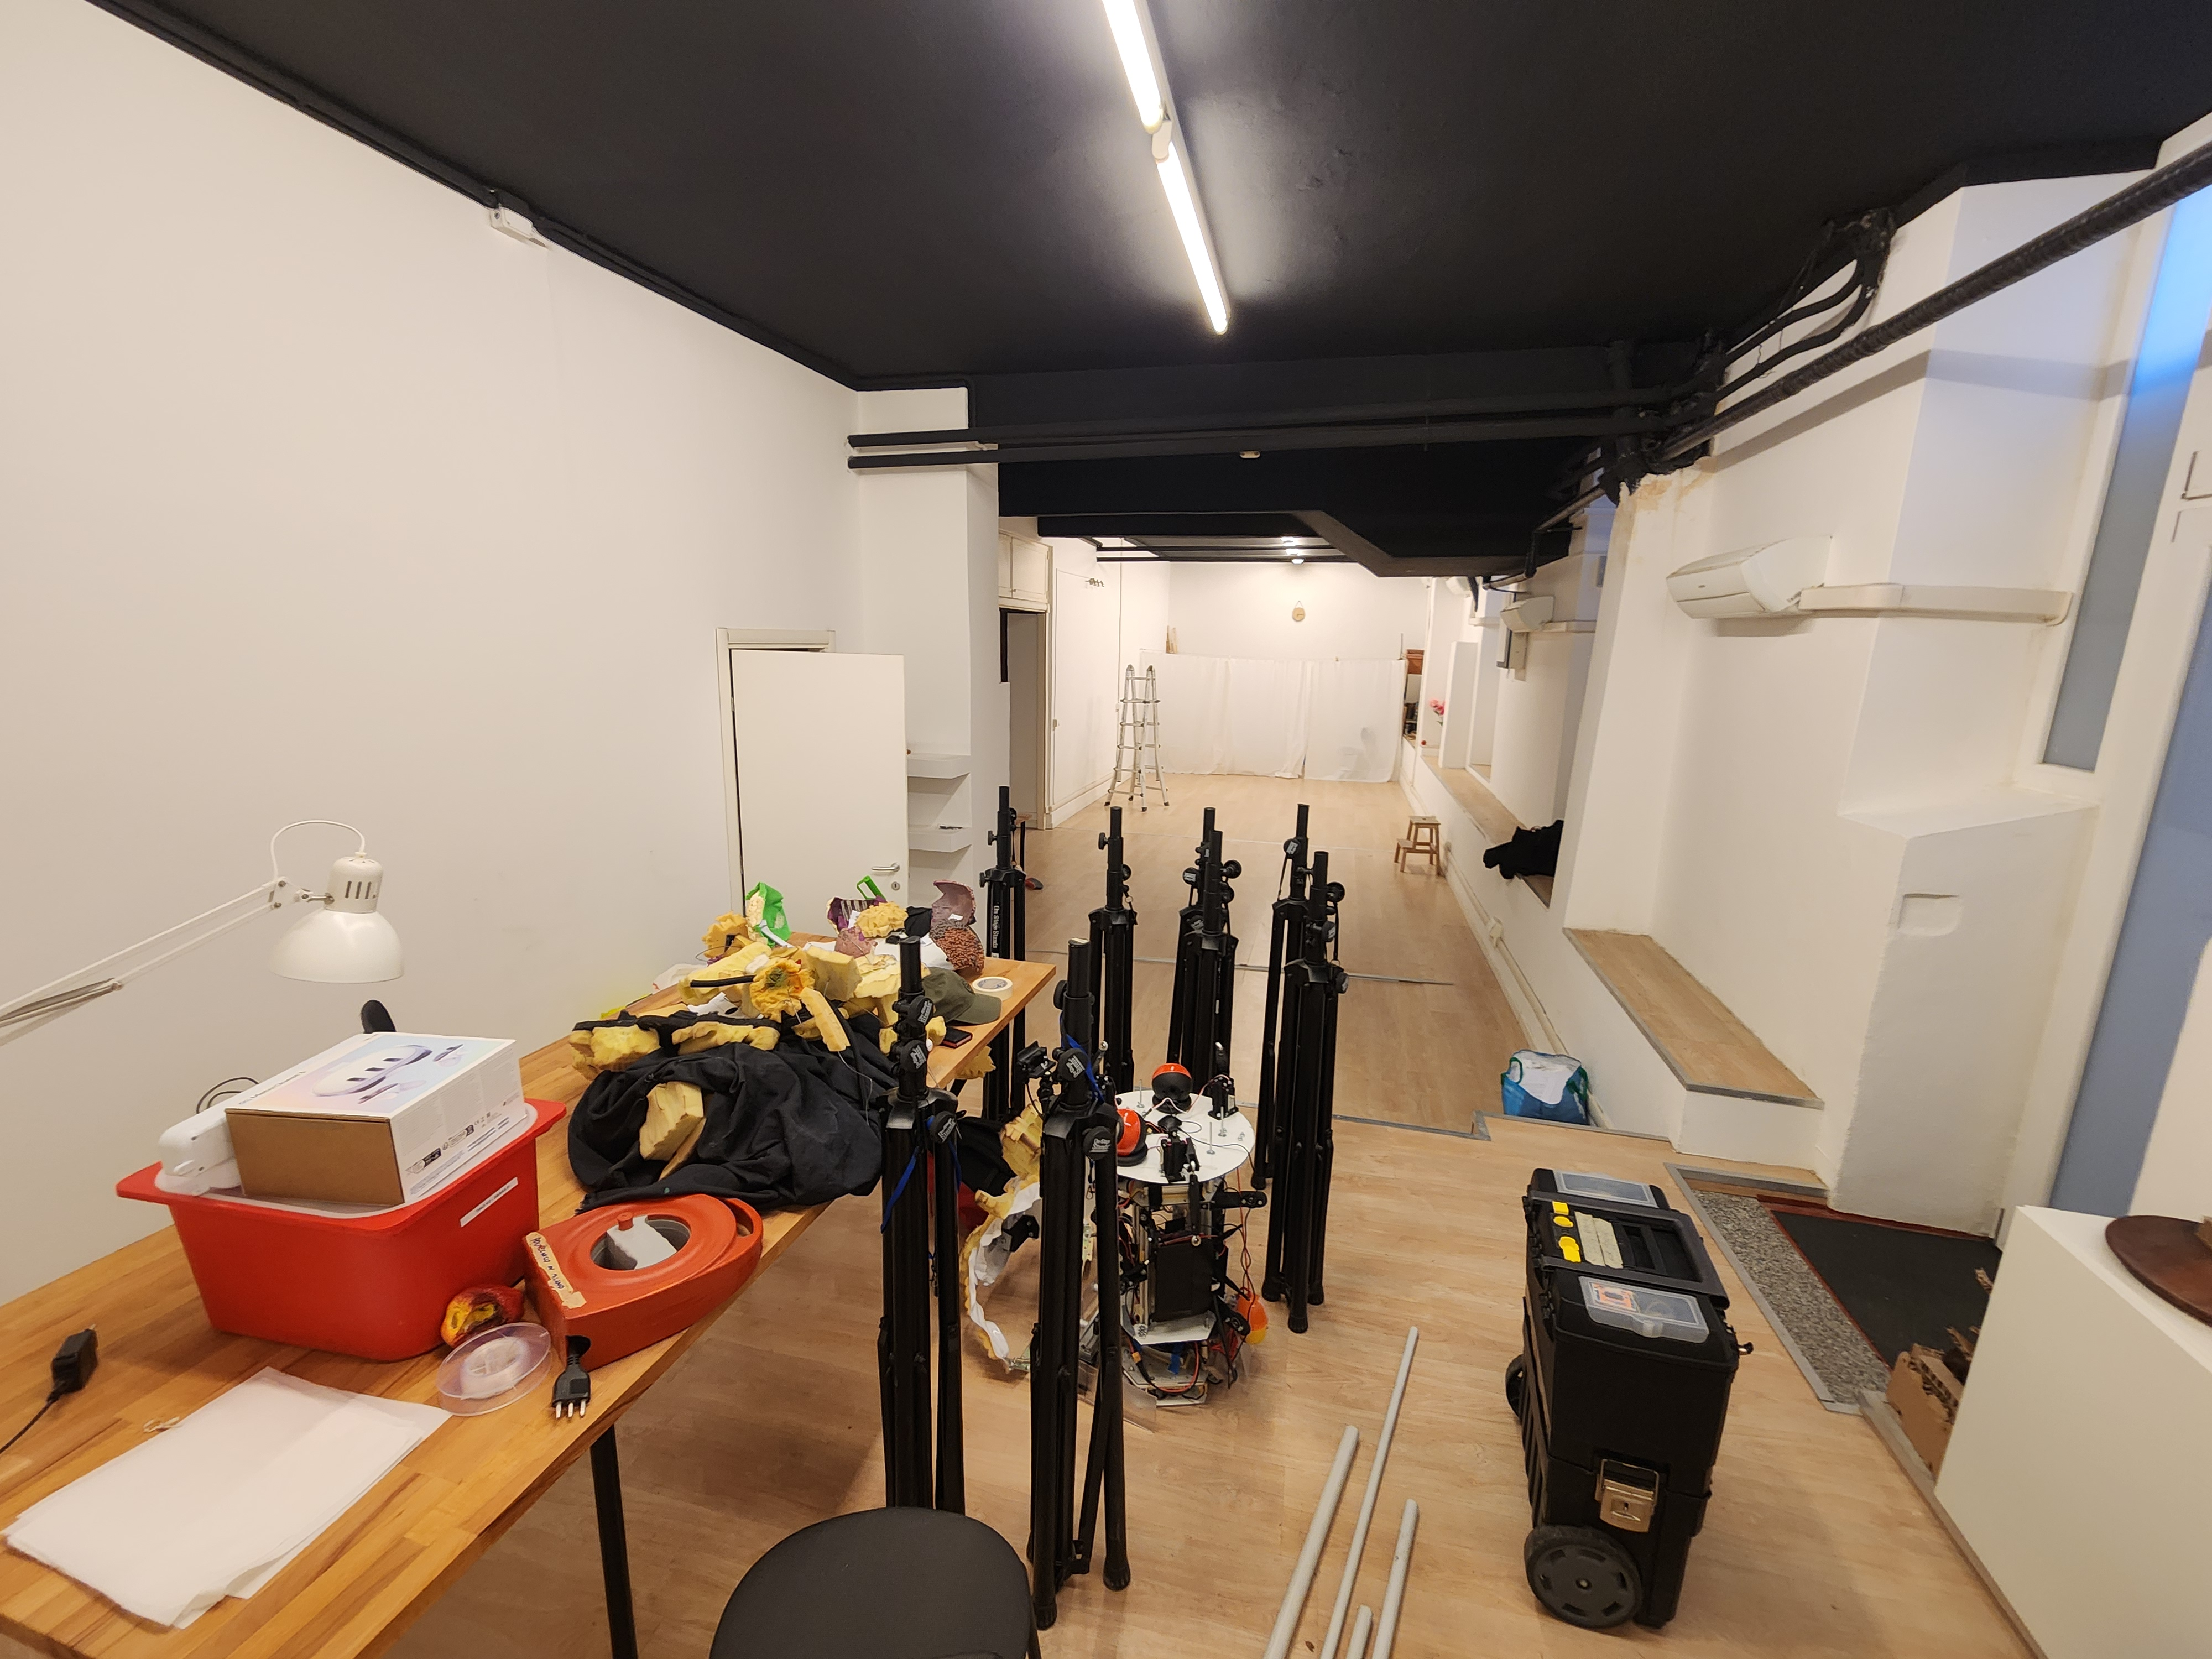
\includegraphics[width=0.9\textwidth]{Images/LabExperimentBefore.jpg}
    \caption{Overview of the Three-Room Experimental Setup}
    \label{fig:lab_experiment_overview}
\end{figure}

The experimental design consists of three sequential areas, each testing progressively complex aspects of VR-mediated human-robot collaboration:

\textbf{Room 1: Spatial Coordination and Platform Alignment}

The largest testing area features two marked platforms positioned at opposite corners. The human participant stands on one platform while Tino, controlled via VR, must navigate to the corresponding robot platform. The critical challenge involves a ``mud'' zone surrounding the human's platform, marked with tape in the physical space but represented as hazardous terrain in the VR environment.

\begin{figure}[H]
    \centering
    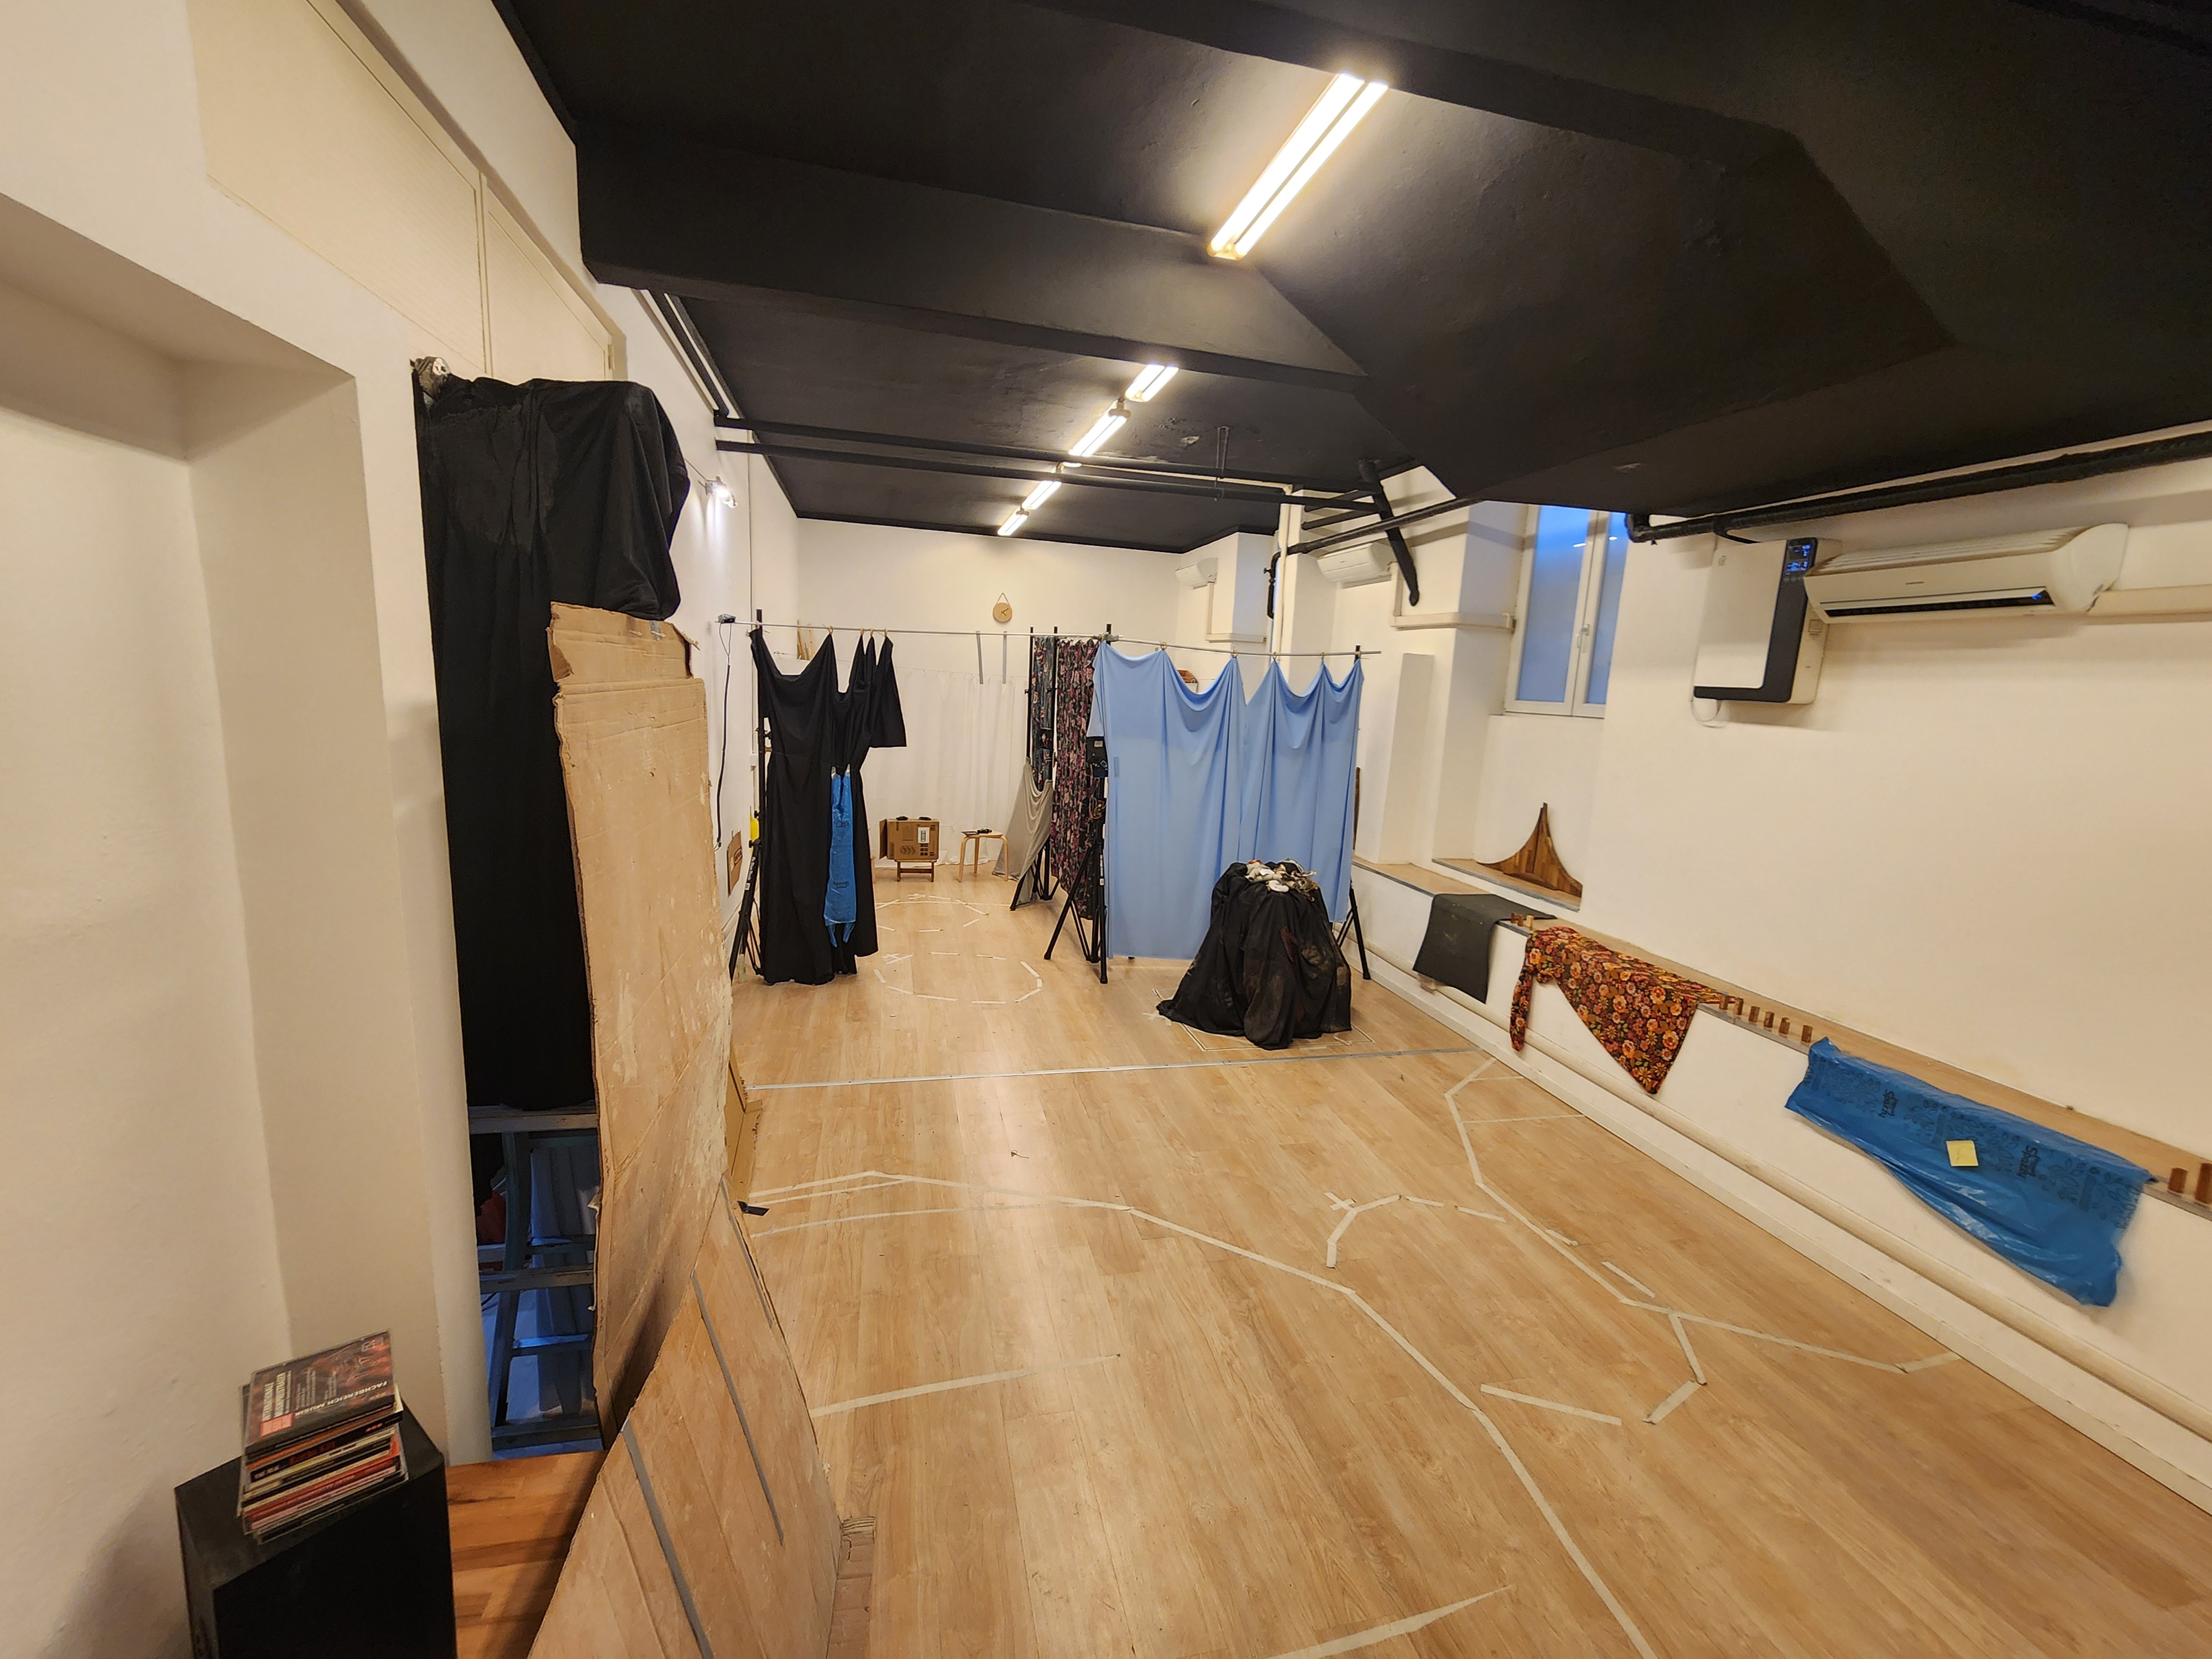
\includegraphics[width=0.8\textwidth]{Images/LabVisualAids (4).jpg}
    \caption{Room 1: Platform Alignment Challenge with Hazard Zones}
    \label{fig:room1_platform_challenge}
\end{figure}

The VR environment includes a custom-designed virtual world that spatially corresponds to the physical testing space in terms of area dimensions, boundary positions, platform locations, and door placements, providing accurate spatial reference for the remote operator. This design tests the hybrid localization system's accuracy and the operator's ability to interpret environmental constraints through VR representation. Success requires non-verbal communication between human participant and VR operator to coordinate simultaneous platform positioning, validating both spatial awareness and collaborative signaling capabilities.

\textbf{Room 2: Information Asymmetry and Communication}

The second area presents a classic information asymmetry scenario where only the VR operator can identify the correct control element among three available options. Three remote controls are positioned within the room, but the human participant cannot determine which one opens the door to the final area.

\begin{figure}[H]
    \centering
    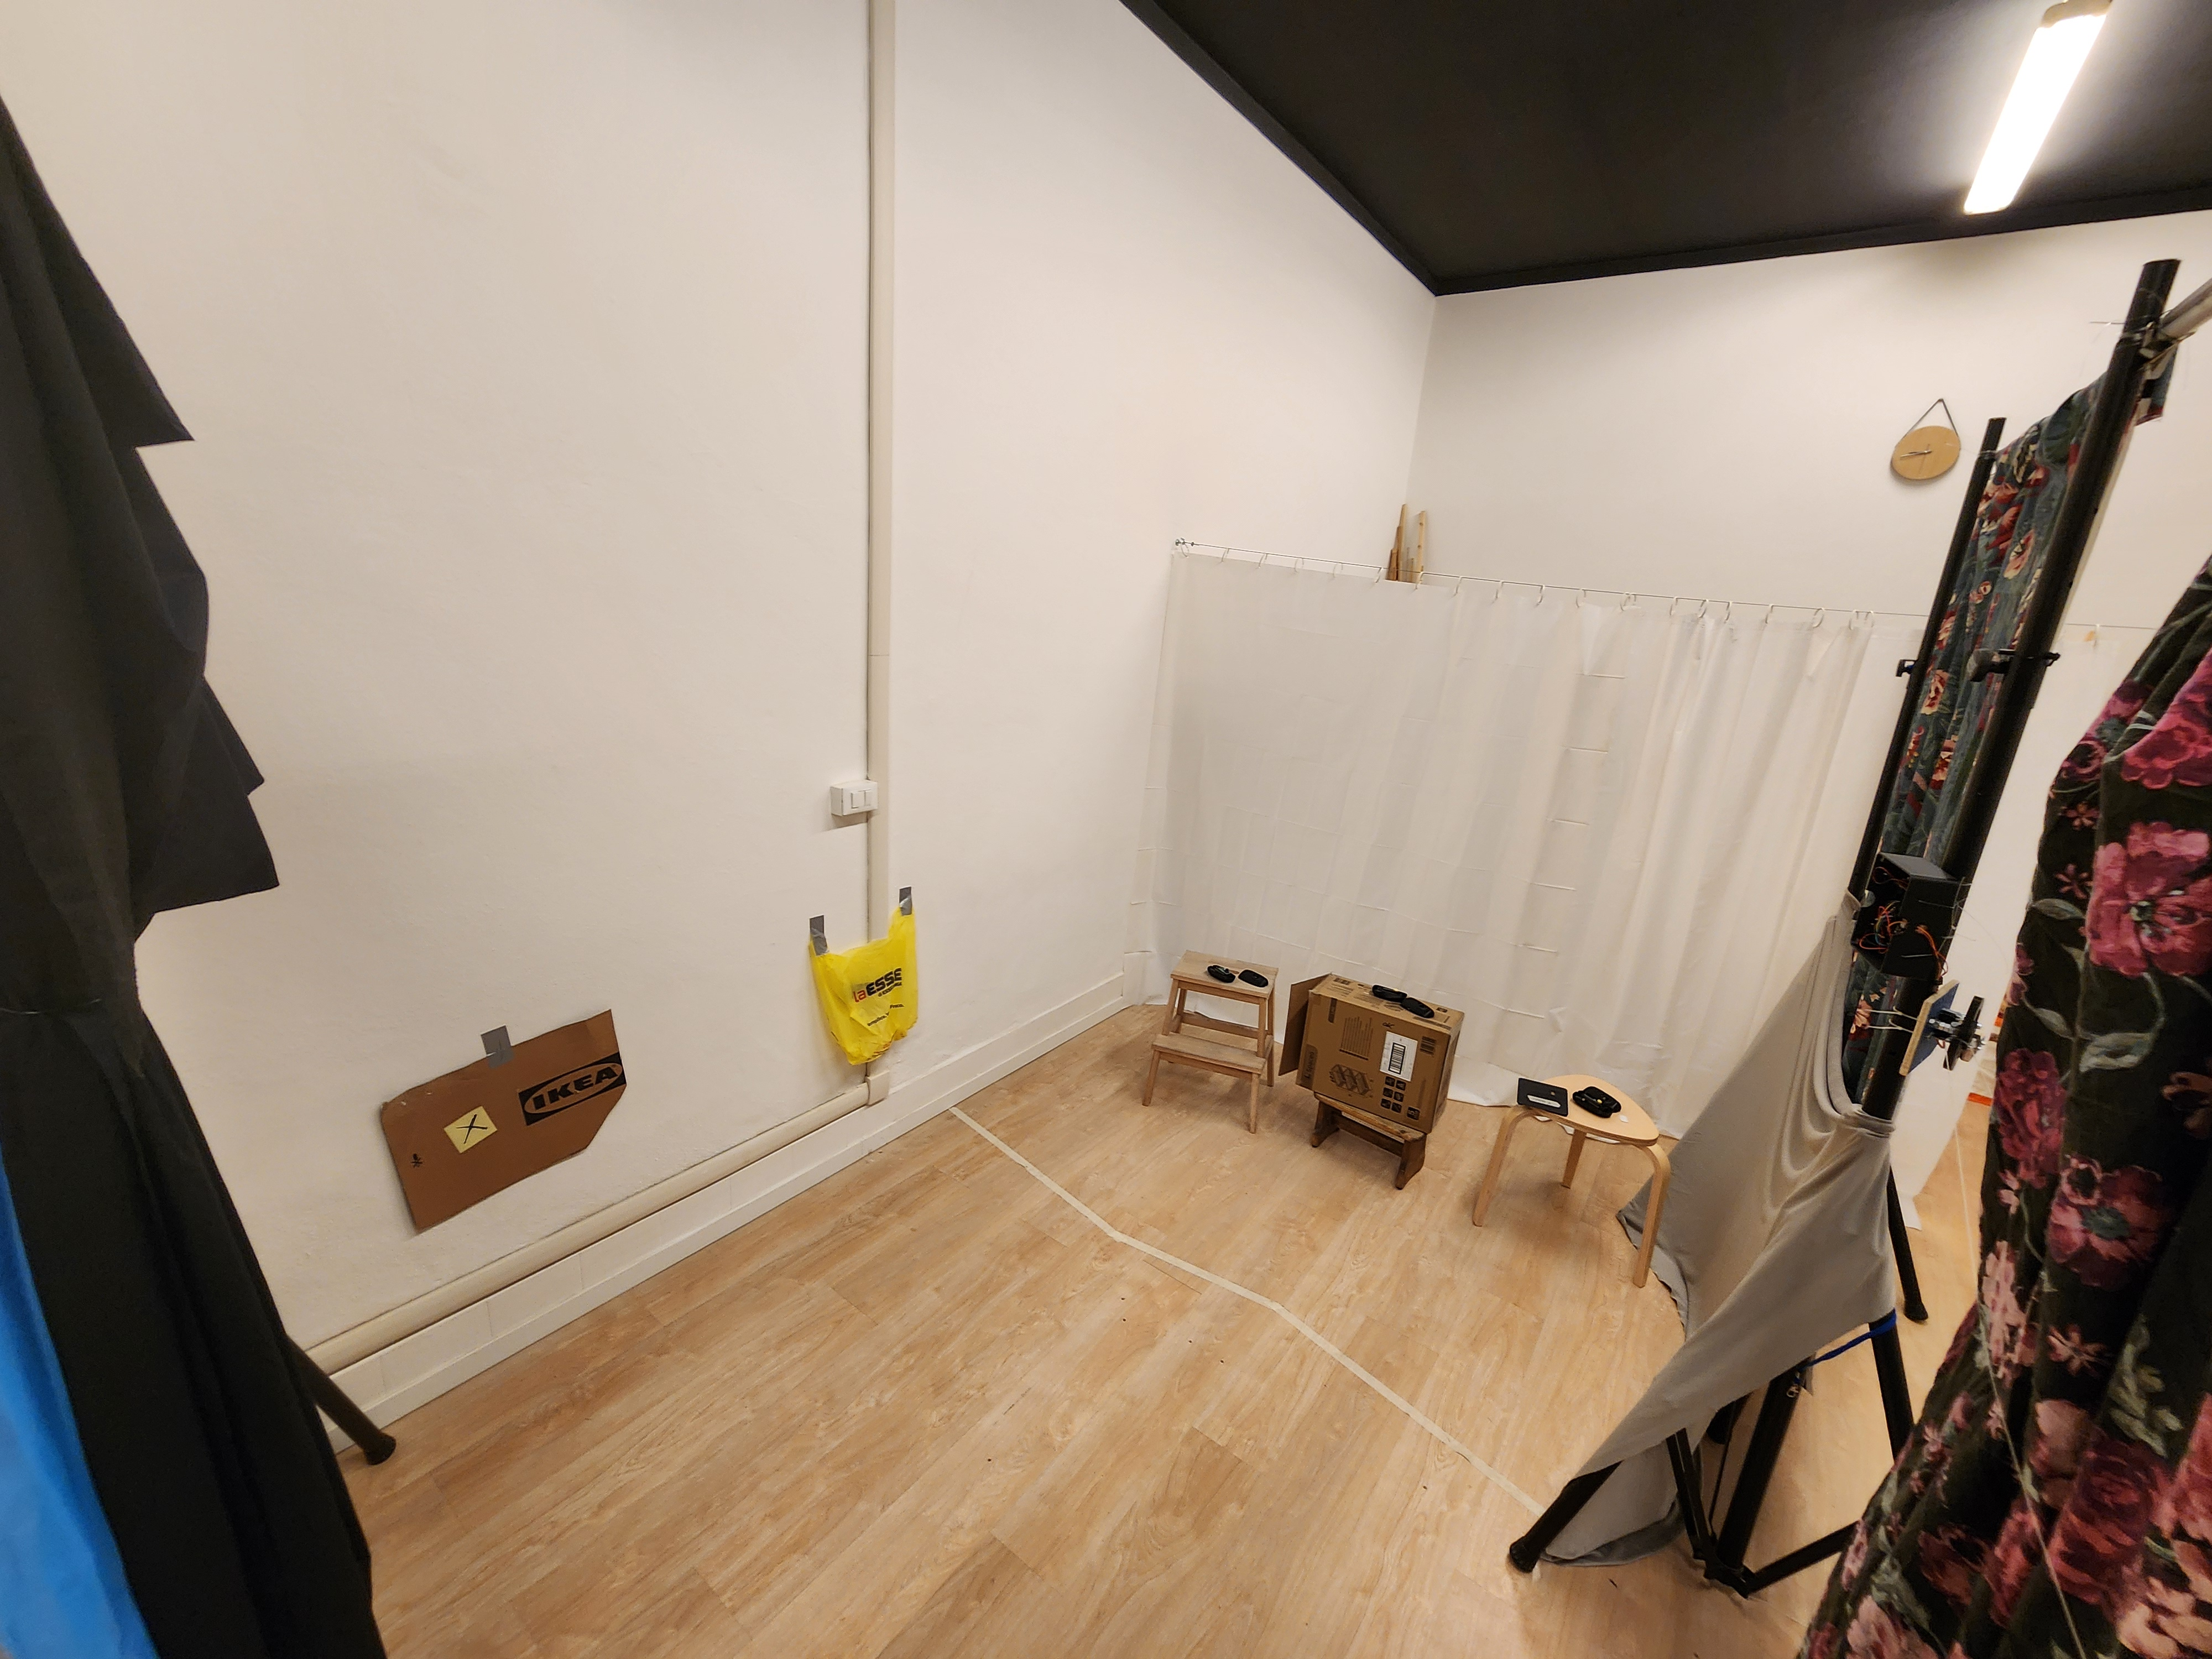
\includegraphics[width=0.8\textwidth]{Images/LabVisualAids (3).jpg}
    \caption{Room 2: Remote Control Selection Challenge}
    \label{fig:room2_remote_challenge}
\end{figure}

This scenario specifically tests the VR operator's ability to convey directional and selection information through Tino's physical movements and positioning. The task requires the development of effective non-verbal communication protocols using only robot movement patterns, head orientation, and spatial positioning. Success depends on the human participant's ability to interpret these movement-based signals and the VR operator's skill in generating clear, consistent communication patterns.

\textbf{Room 3: Temporal Coordination and Completion}

The final area serves as both the completion zone and a test of empathy and coordination under time pressure. While appearing as a simple ``victory'' room, the true challenge requires the human participant to wait for Tino to cross the threshold before claiming success.

This design tests several critical aspects: the VR operator's awareness of collaborative requirements, their ability to communicate urgency or completion needs through robot behavior, and the system's capacity to maintain engagement and coordination throughout the complete experimental sequence. The temporal aspect introduces pressure that reveals the robustness of the communication patterns established in previous rooms.

\subsection{VR Hardware and Setup}

The VR testing setup utilizes Unity-based immersive environments integrated with the ROS2 communication architecture detailed in Chapter~\ref{sec:software_arch}. Participants operate through commercial VR headsets with dedicated control systems that translate user intentions into atomic movement commands via the standardized VR interface nodes.

The VR environment provides real-time feedback through multiple information channels:

\textbf{Spatial Positioning}: Real-time robot location overlay derived from the hybrid UWB-RTABMap fusion system, enabling operators to maintain spatial awareness during teleoperation.

\textbf{Perception Data}: Live human detection information from the YOLOv11 pose estimation system, allowing VR operators to understand environmental context and human presence during collaborative tasks.

\textbf{Movement Feedback}: Direct feedback on atomic movement execution and completion status, enabling VR operators to understand when commanded actions have been successfully completed by the physical robot.

\textbf{Environmental Feedback}: Visual and auditory cues corresponding to physical robot interactions, maintaining immersive connection between VR operator actions and physical robot responses.

\subsection{Task Structure and Evaluation Metrics}

The evaluation methodology focuses on technical system performance indicators that validate the integrated VR teleoperation platform's core capabilities. The three-room experimental sequence exercises all system components simultaneously while providing opportunities to emphasize specific technical evaluations in each environment.

\textbf{Room 1: Platform Alignment Challenge} (15 minutes)
The large-area navigation scenario provides optimal conditions for evaluating localization system performance. While all systems remain active, this room particularly emphasizes hybrid UWB-RTABMap positioning accuracy, coordinate frame alignment between physical and VR environments, and spatial correspondence precision. Technical metrics include absolute positioning error (target: <15cm), localization drift over time, hazard zone boundary detection accuracy, and VR spatial mapping effectiveness.

\textbf{Room 2: VR Communication and Control Precision} (10 minutes)
The information asymmetry scenario, while requiring all system components, creates demanding conditions for evaluating VR communication robustness and atomic movement precision. With the need for precise directional communication and accurate positioning relative to multiple objects, this room emphasizes command transmission reliability, movement execution accuracy, and VR control responsiveness. Technical evaluation focuses on command-response latency, atomic movement completion rates, positioning precision near target objects, and communication stability during intensive control sequences.

\textbf{Room 3: Human Pose Detection and Tracking} (5 minutes)
The completion coordination scenario exercises the complete system while providing concentrated evaluation of human detection and pose estimation capabilities. As the VR operator must understand human participant positioning and movement to coordinate completion timing, this room emphasizes YOLOv11 detection accuracy, pose tracking consistency, and real-time human state interpretation. Technical metrics include detection reliability during varied human positions, pose estimation accuracy, and processing performance during critical coordination moments.

Throughout all rooms, comprehensive system integration performance is monitored, including overall reliability, inter-component coordination, and sustained operation characteristics. Each room provides focused evaluation opportunities while maintaining complete system validation across the entire experimental sequence.

\section{Experimental Results and Analysis}
\label{sec:experimental_results}

Evaluation testing was conducted over five consecutive days with twelve volunteer participants, providing comprehensive data on system performance across diverse user experience levels and interaction styles. The participant group included individuals with varying VR experience (ranging from novice to expert), robotics familiarity, and technical backgrounds to ensure representative evaluation of system accessibility and usability.

\subsection{VR Control System Performance}

The atomic movement framework demonstrated robust technical reliability in command transmission and execution throughout all testing scenarios. Command reception and processing achieved near-perfect reliability, with the vast majority of VR-initiated commands successfully transmitted through the ROS2-Unity communication bridge and properly executed by the hardware interface systems. Occasional command losses (less than 2\% of total commands) were observed during testing, most likely attributed to network packet loss in the Unity-ROS2 communication bridge during high-traffic scenarios.

\begin{table}[H]
    \centering
    \footnotesize
    \begin{tabular}{|p{3cm}|p{1.8cm}|p{1.8cm}|p{1.8cm}|}
        \hline
        \textbf{Movement Type} & \textbf{Command Success (\%)} & \textbf{Avg Response (s)} & \textbf{Execution Reliability (\%)} \\
        \hline
        Forward Movement & 98.7 & 1.73 & 98.4 \\
        Rotation (Left/Right) & 98.3 & 1.85 & 97.8 \\
        Leg Coordination & 98.1 & 2.15 & 94.6 \\
        Combined Movements & 98.9 & 2.82 & 96.2 \\
        \hline
    \end{tabular}
    \caption{VR Control System Technical Performance Metrics}
    \label{tab:vr_control_performance}
\end{table}

The pulse-based command system proved particularly effective in preventing command accumulation and ensuring predictable robot responses. The 3-cycle pulse generation mechanism successfully eliminated timing conflicts and provided reliable command-to-execution correspondence throughout testing sessions.

User feedback from the experimental sessions corroborated the technical performance findings, with 67\% of participants reporting difficulties with movement controls, particularly citing slow response times and movement precision challenges. Comments such as ``Tino era davvero molto lento'' (Tino was really very slow) and complaints about ``movement inputs'' directly aligned with the identified limitations in atomic movement timing constraints.

Critical technical findings include:

\textbf{Movement Completion Reliability}: The atomic movement system's completion guarantee eliminated partial movement issues that could compromise task performance. No instances of incomplete movements were recorded during testing, validating the 4-state coordination approach and confirming reliable hardware-software integration.

\textbf{Timing Consistency}: The standardized 1.7-second movement duration for coordinated actions provided predictable system behavior with consistent execution timing across all test sessions, demonstrating robust temporal coordination between base and leg controllers.

\textbf{Hardware Performance Limitations}: Testing revealed a notable vibration issue in the leg mechanism during State 2 (maximum extension hold position). The leg actuator exhibited significant oscillation when maintaining maximum elevation, indicating suboptimal PID tuning parameters and mechanical stress from supporting leg weight at full extension. This vibration did not affect movement completion but suggests optimization opportunities for control system refinement.

\subsection{Localization and Spatial Awareness}

Prior to conducting the full VR teleoperation experiments, extensive localization system validation was performed to establish the accuracy and reliability requirements for spatial awareness during collaborative tasks. This comprehensive evaluation began with environmental mapping and progressed through baseline testing using RTABMap-only localization before implementing the hybrid positioning approach.

\textbf{Environmental Mapping and Preparation}

The initial phase of localization system evaluation required the creation of a comprehensive 3D map of the experimental environment using RTABMap's visual SLAM capabilities. This mapping process proved essential for subsequent localization accuracy and represented a significant preparatory phase of the evaluation.

\begin{figure}[H]
    \centering
    \begin{minipage}{0.48\textwidth}
        \centering
        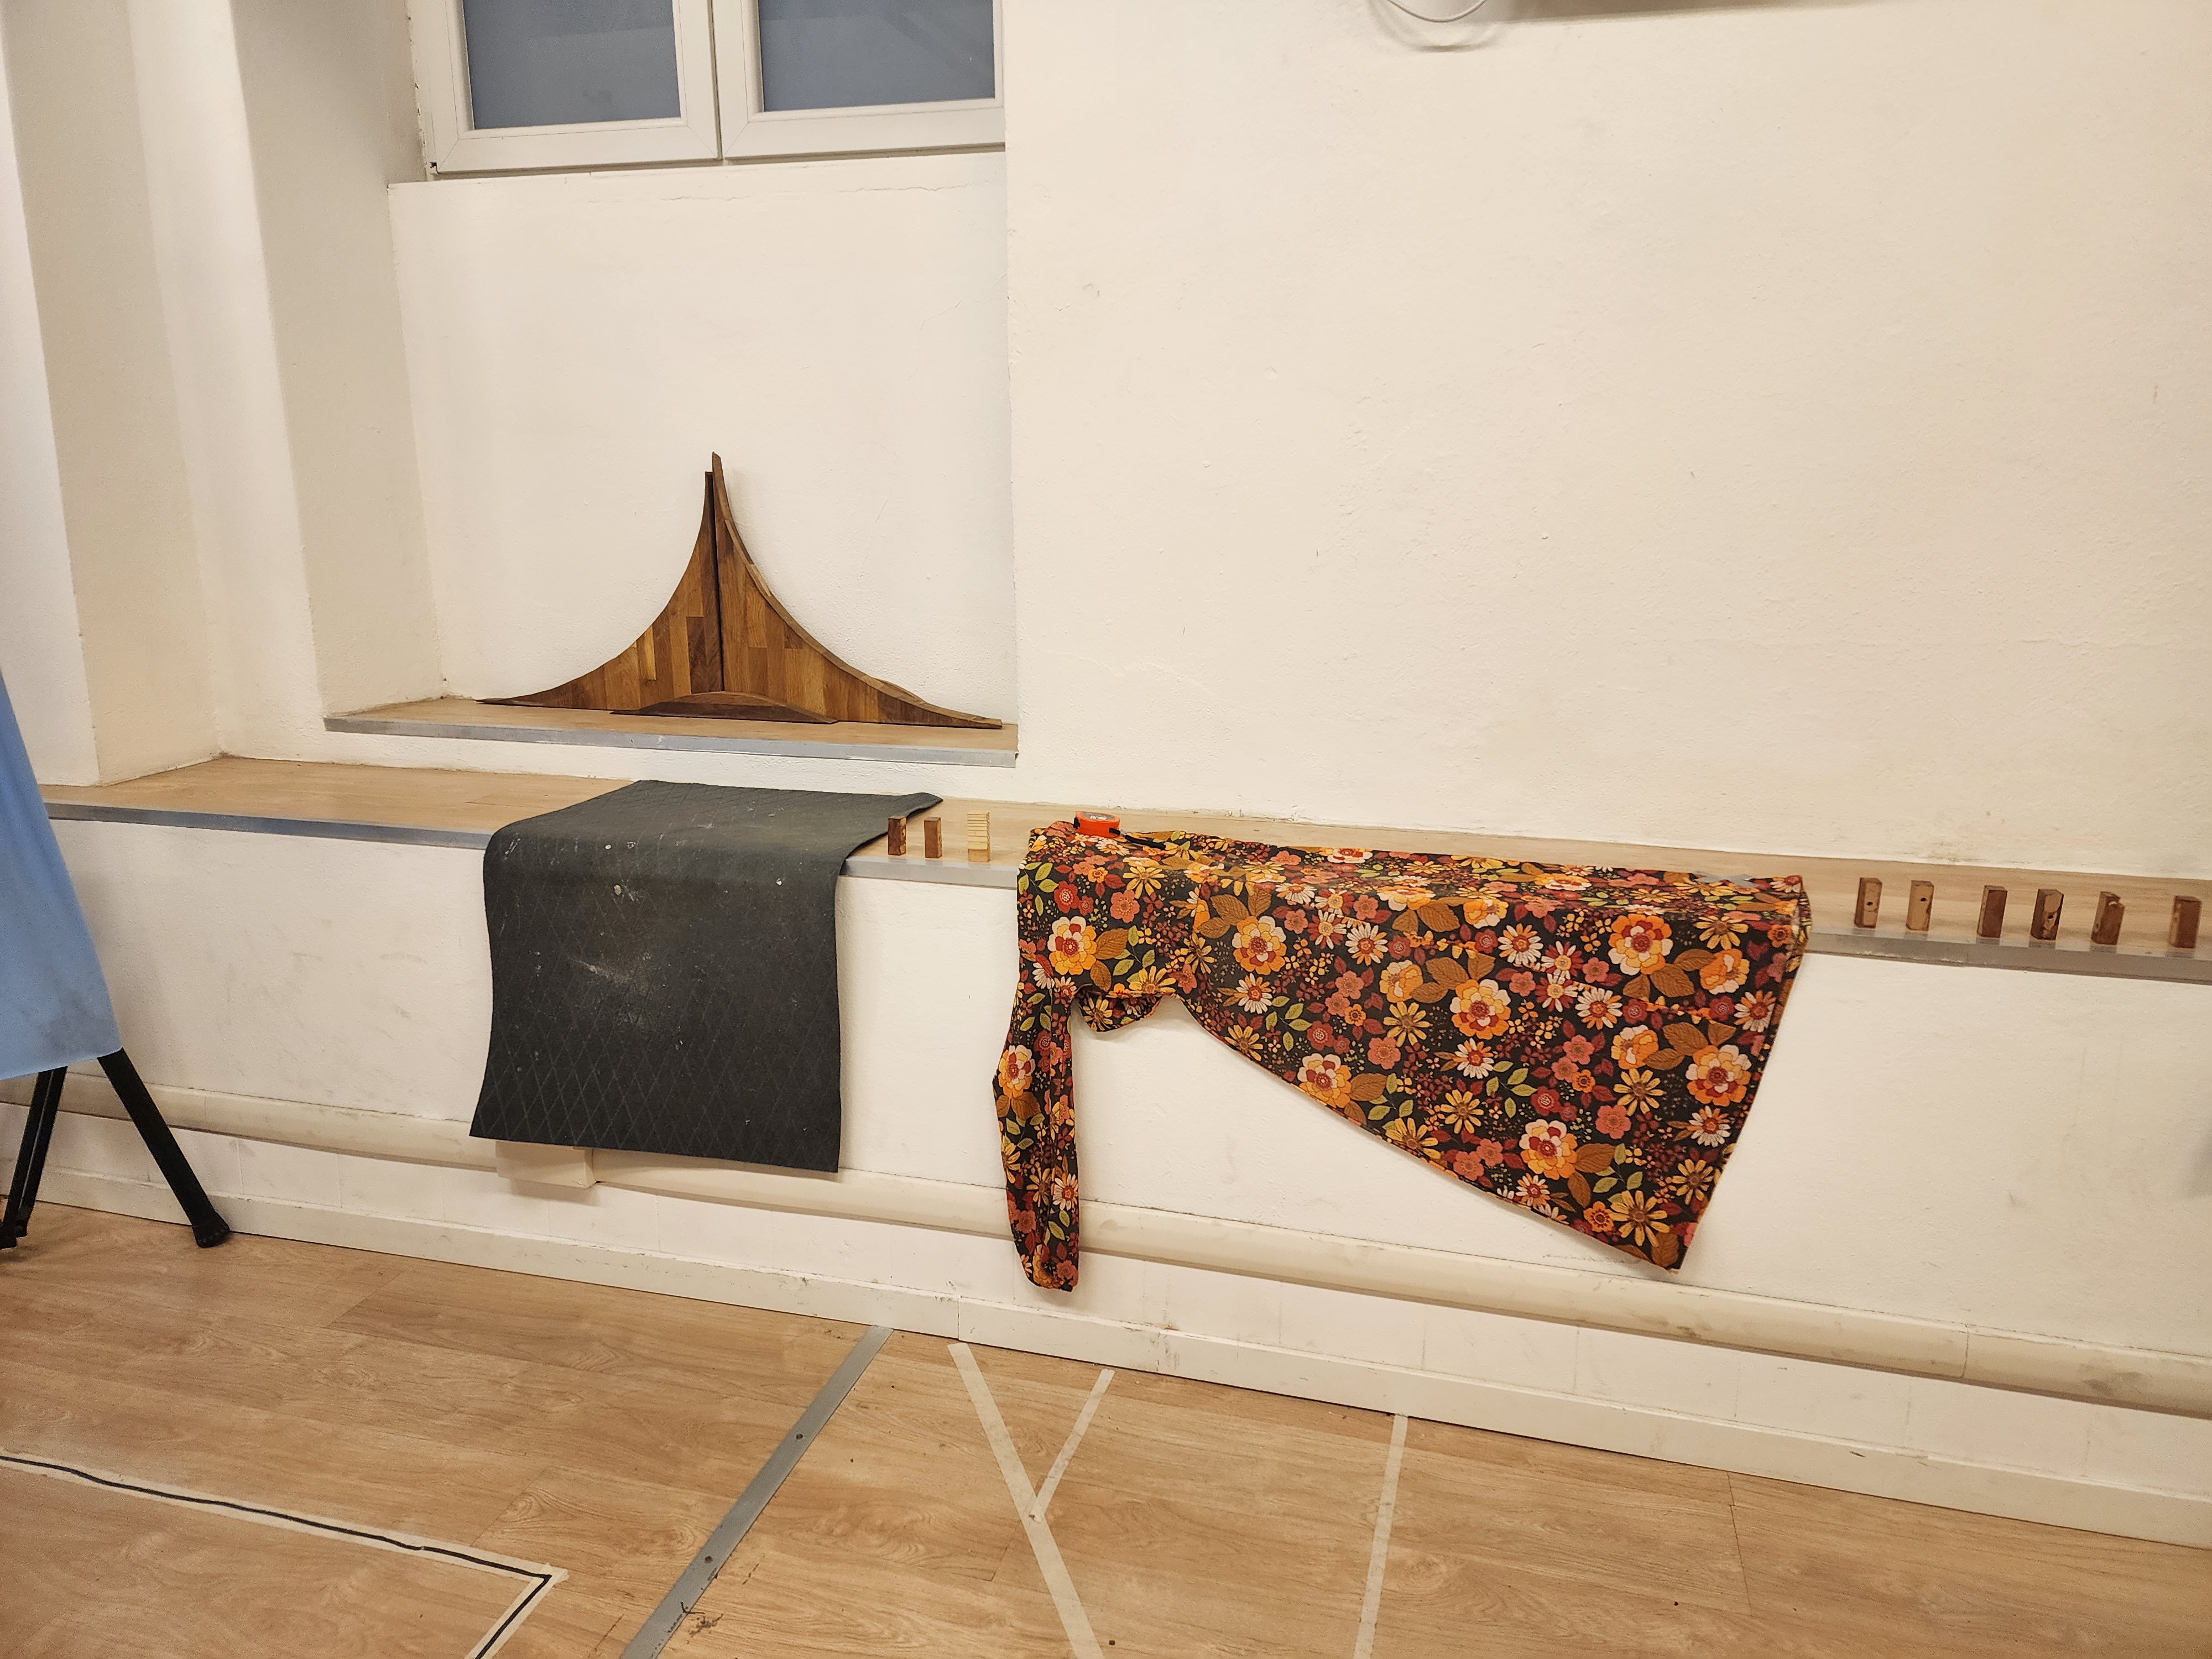
\includegraphics[width=\textwidth]{Images/LabVisualAids (6).jpg}
        \caption{Wall-mounted Visual References}
        \label{fig:lab_wall_features}
    \end{minipage}
    \hfill
    \begin{minipage}{0.48\textwidth}
        \centering
        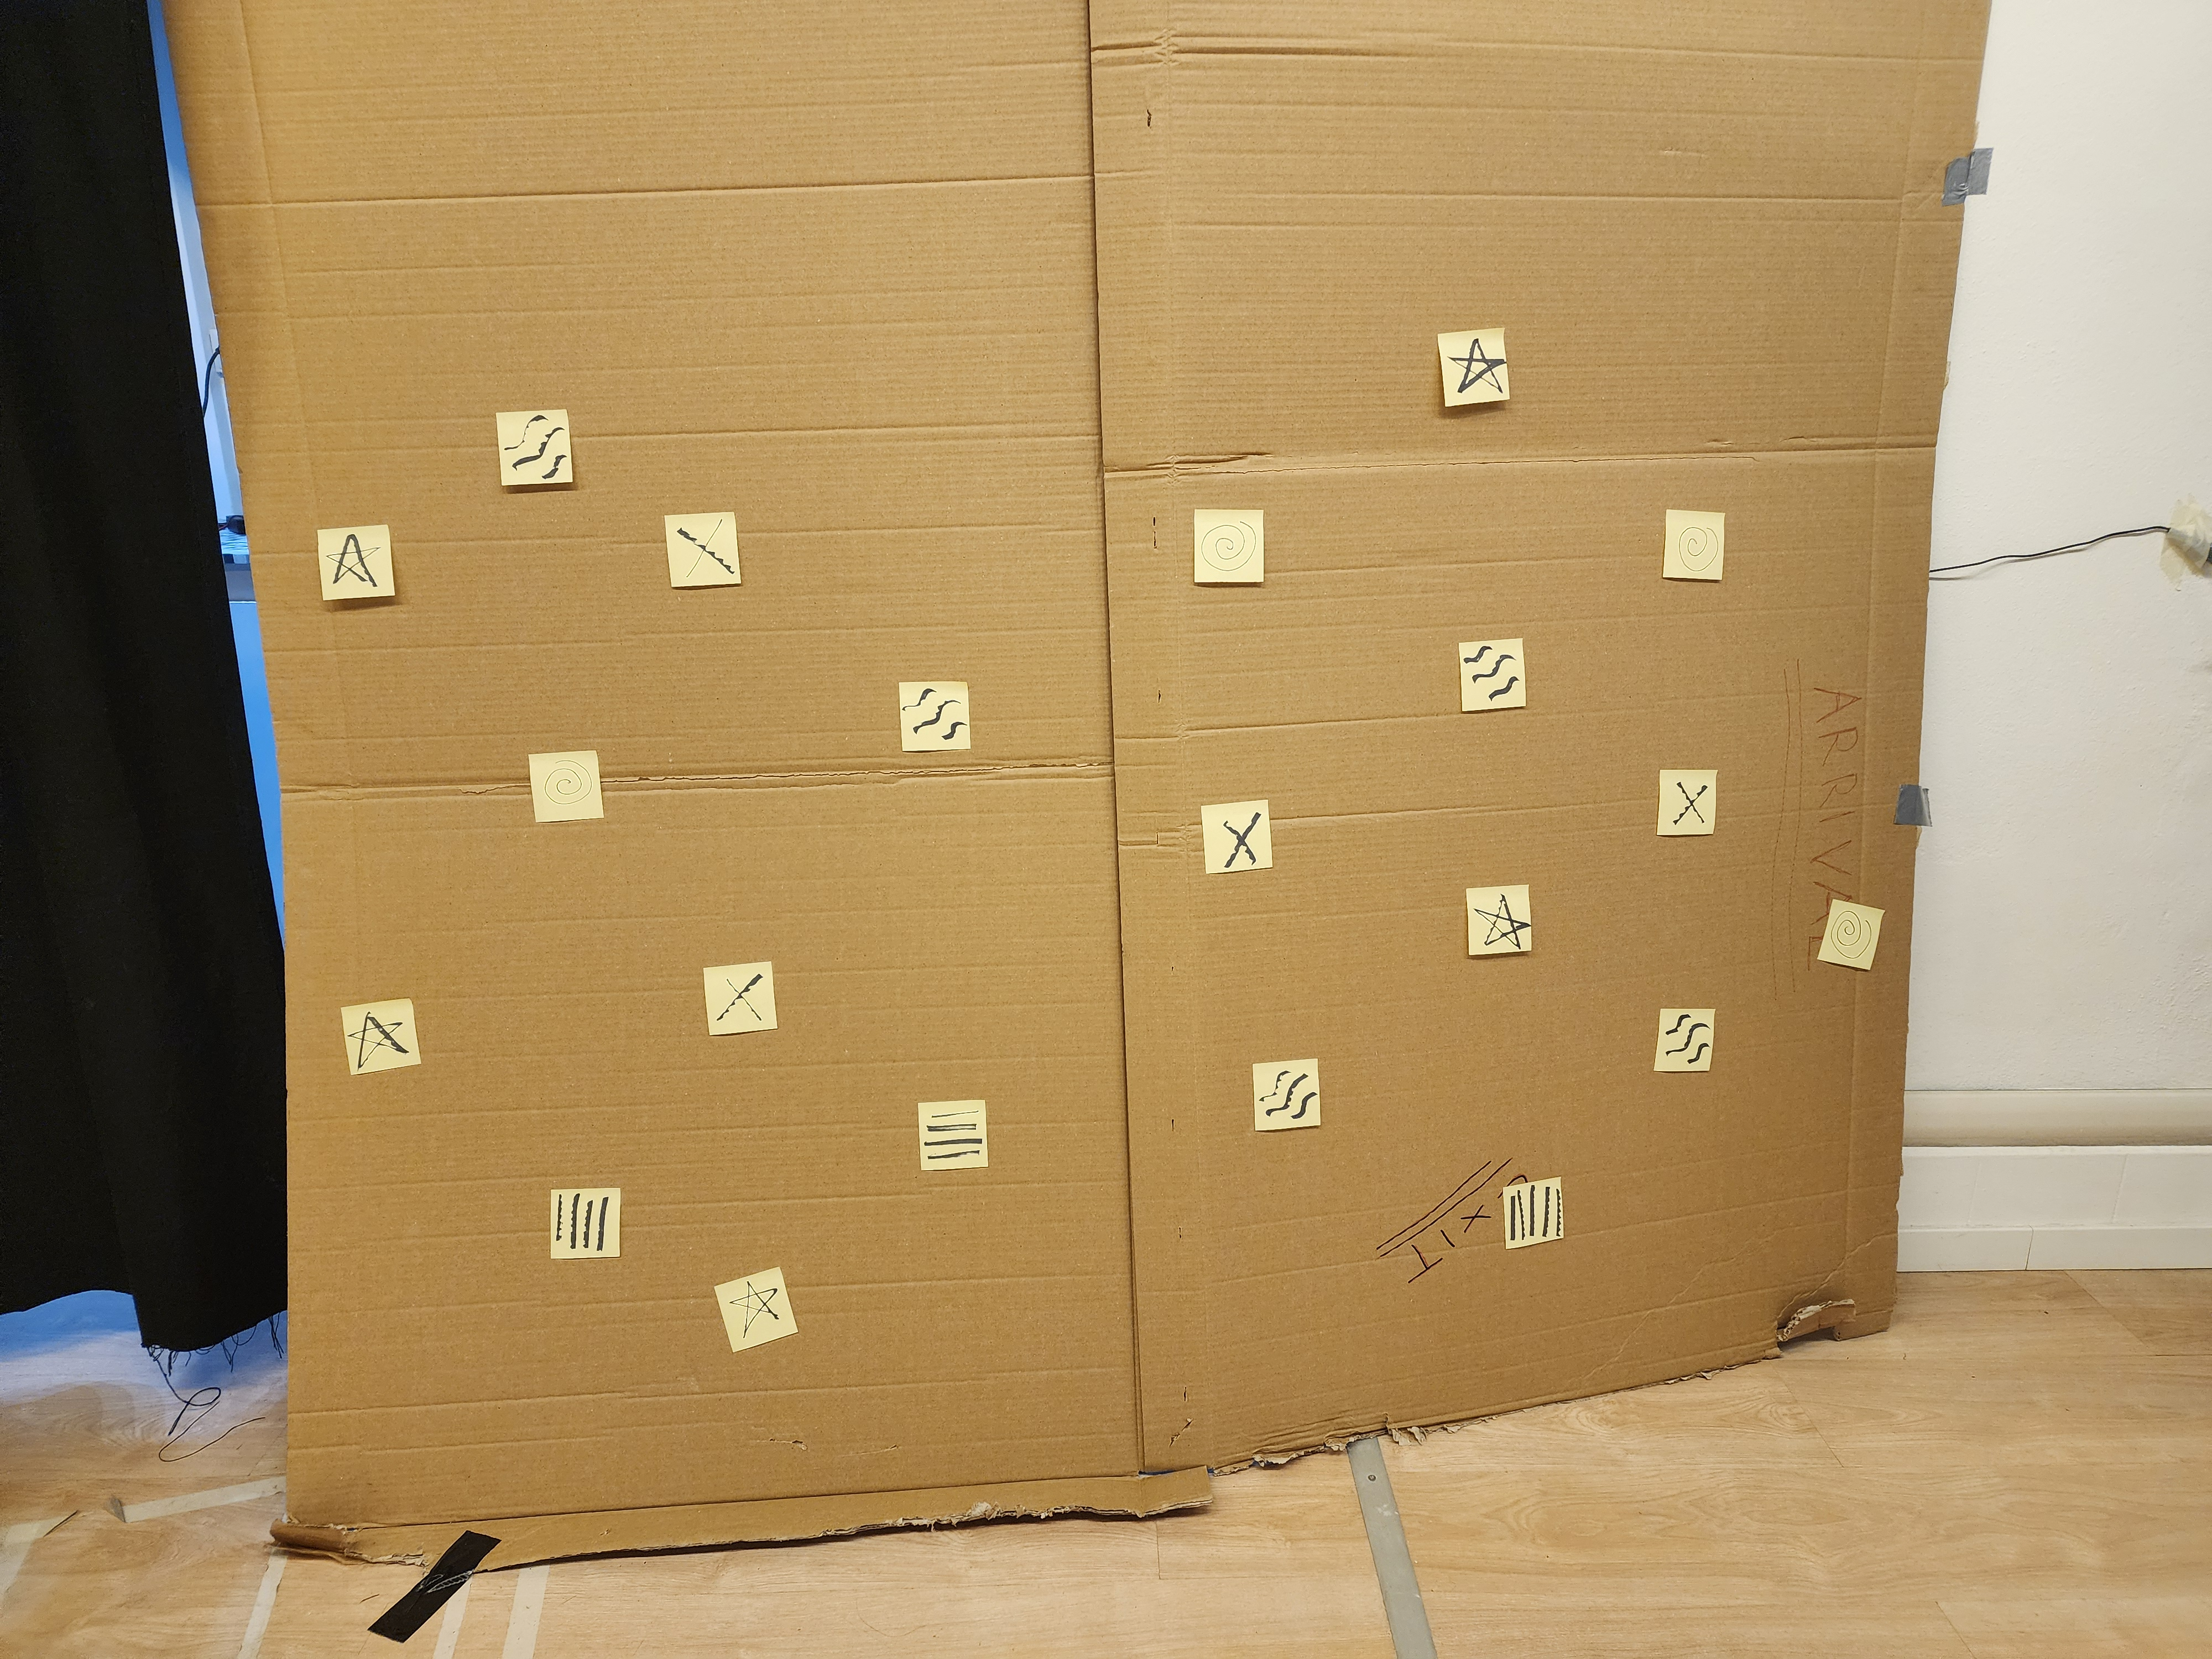
\includegraphics[width=\textwidth]{Images/LabVisualAids (2).jpg}
        \caption{Post-it Notes and Markers for SLAM Enhancement}
        \label{fig:lab_postit_features}
    \end{minipage}
\end{figure}

The mapping process required approximately 1.5 hours of systematic navigation throughout the experimental area to achieve comprehensive coverage. Initial mapping attempts revealed insufficient visual features in certain laboratory areas, particularly near uniform walls and open spaces, necessitating strategic placement of visual landmarks to improve SLAM performance.

\begin{figure}[H]
    \centering
    \begin{minipage}{0.32\textwidth}
        \centering
        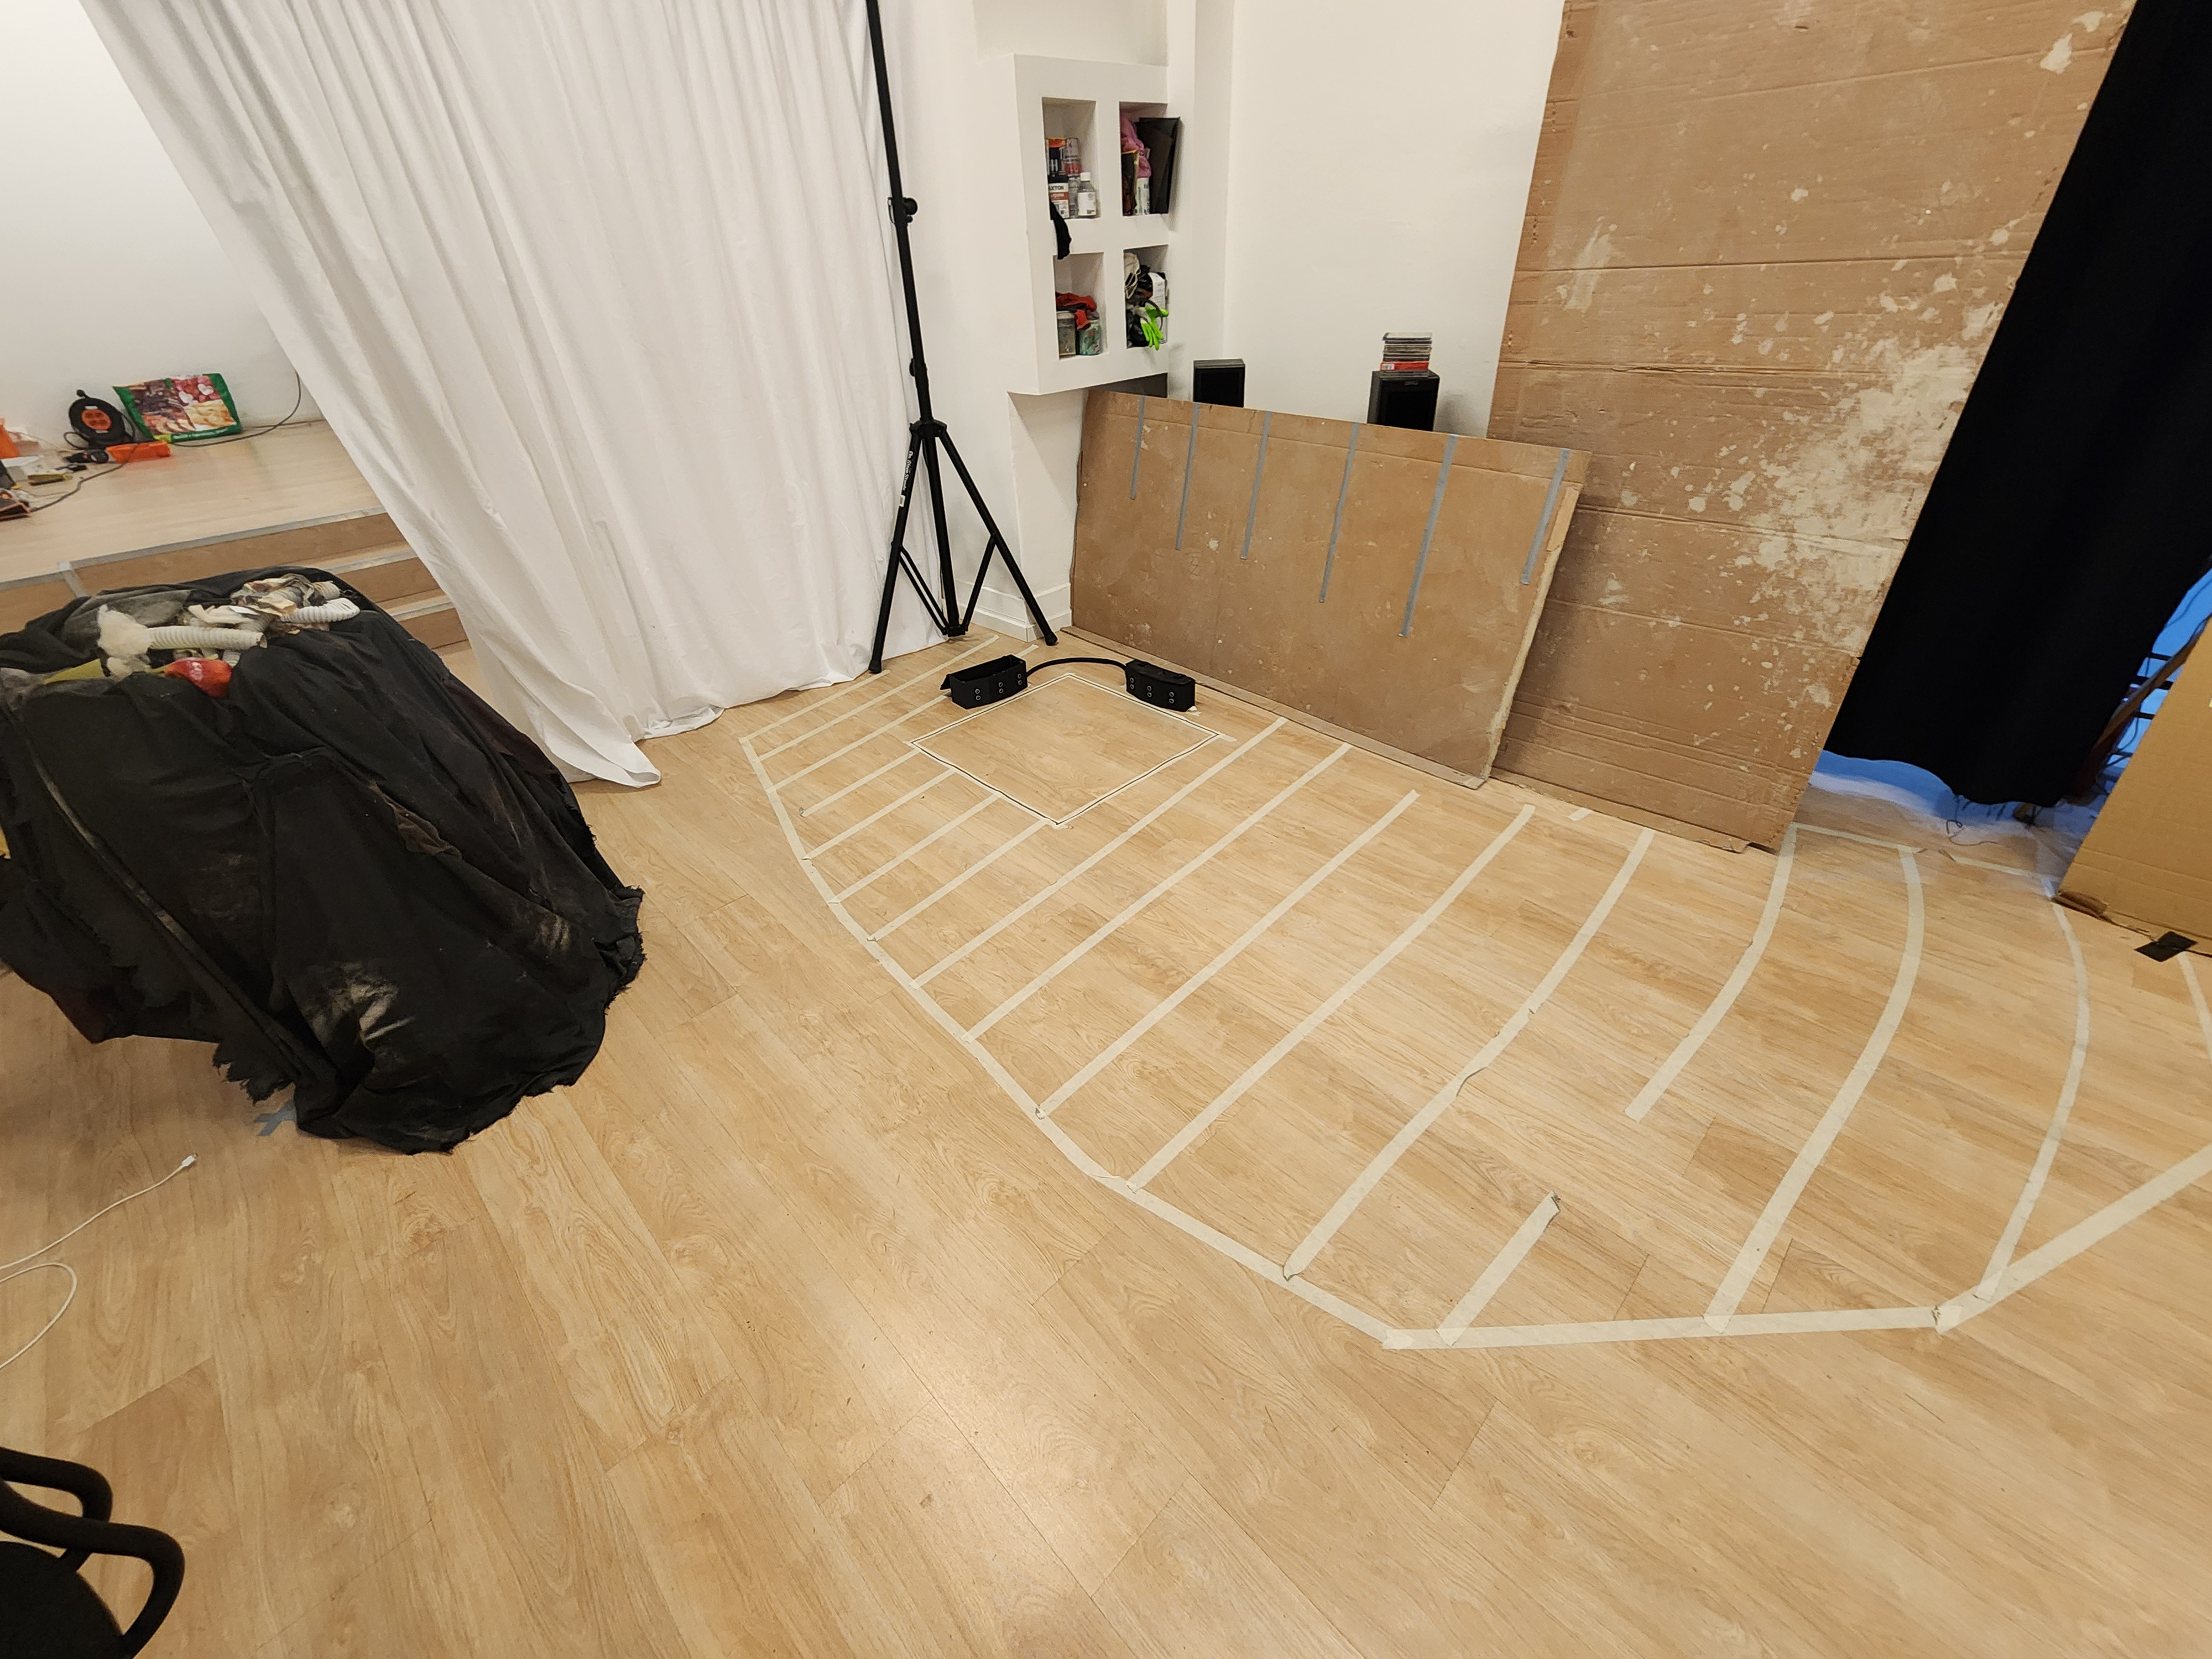
\includegraphics[width=\textwidth]{Images/LabVisualAids (5).jpg}
        \caption{Corner Area Feature Enhancement}
        \label{fig:corner_features}
    \end{minipage}
    \hfill
    \begin{minipage}{0.32\textwidth}
        \centering
        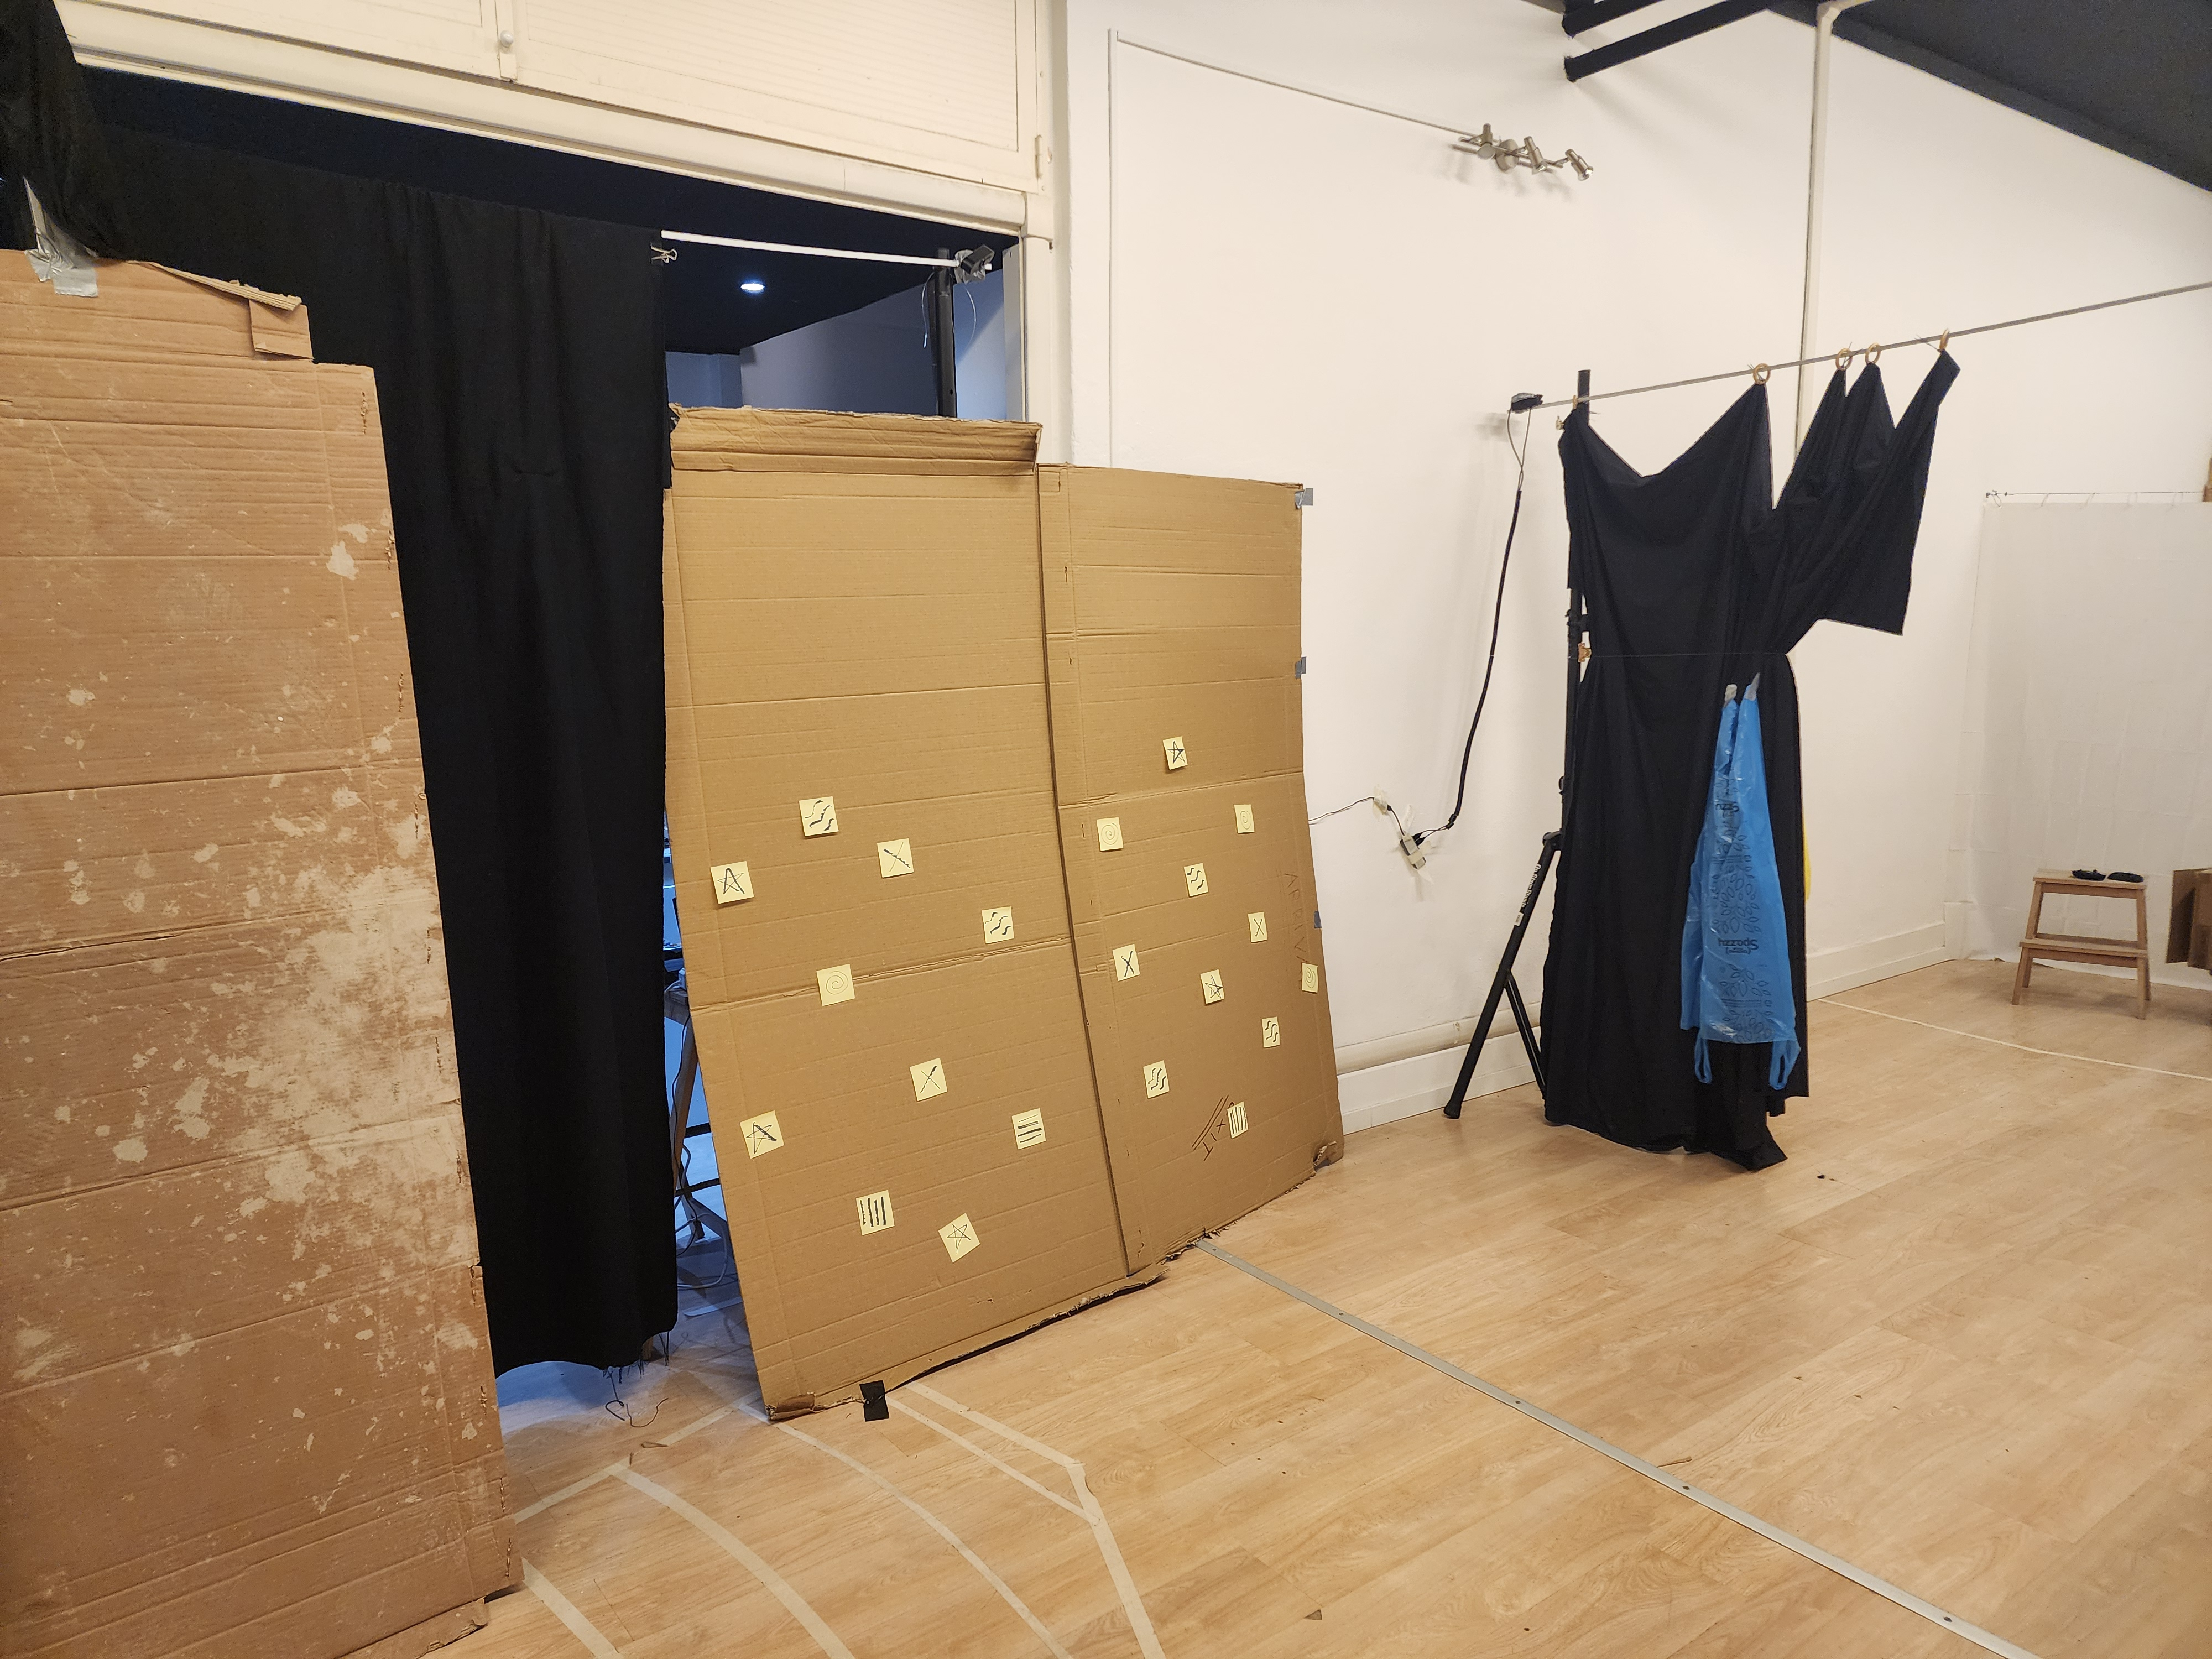
\includegraphics[width=\textwidth]{Images/LabVisualAids.jpg}
        \caption{Door corner with Visual Markers}
        \label{fig:door_corner_features}
    \end{minipage}
    \hfill
    \begin{minipage}{0.32\textwidth}
        \centering
        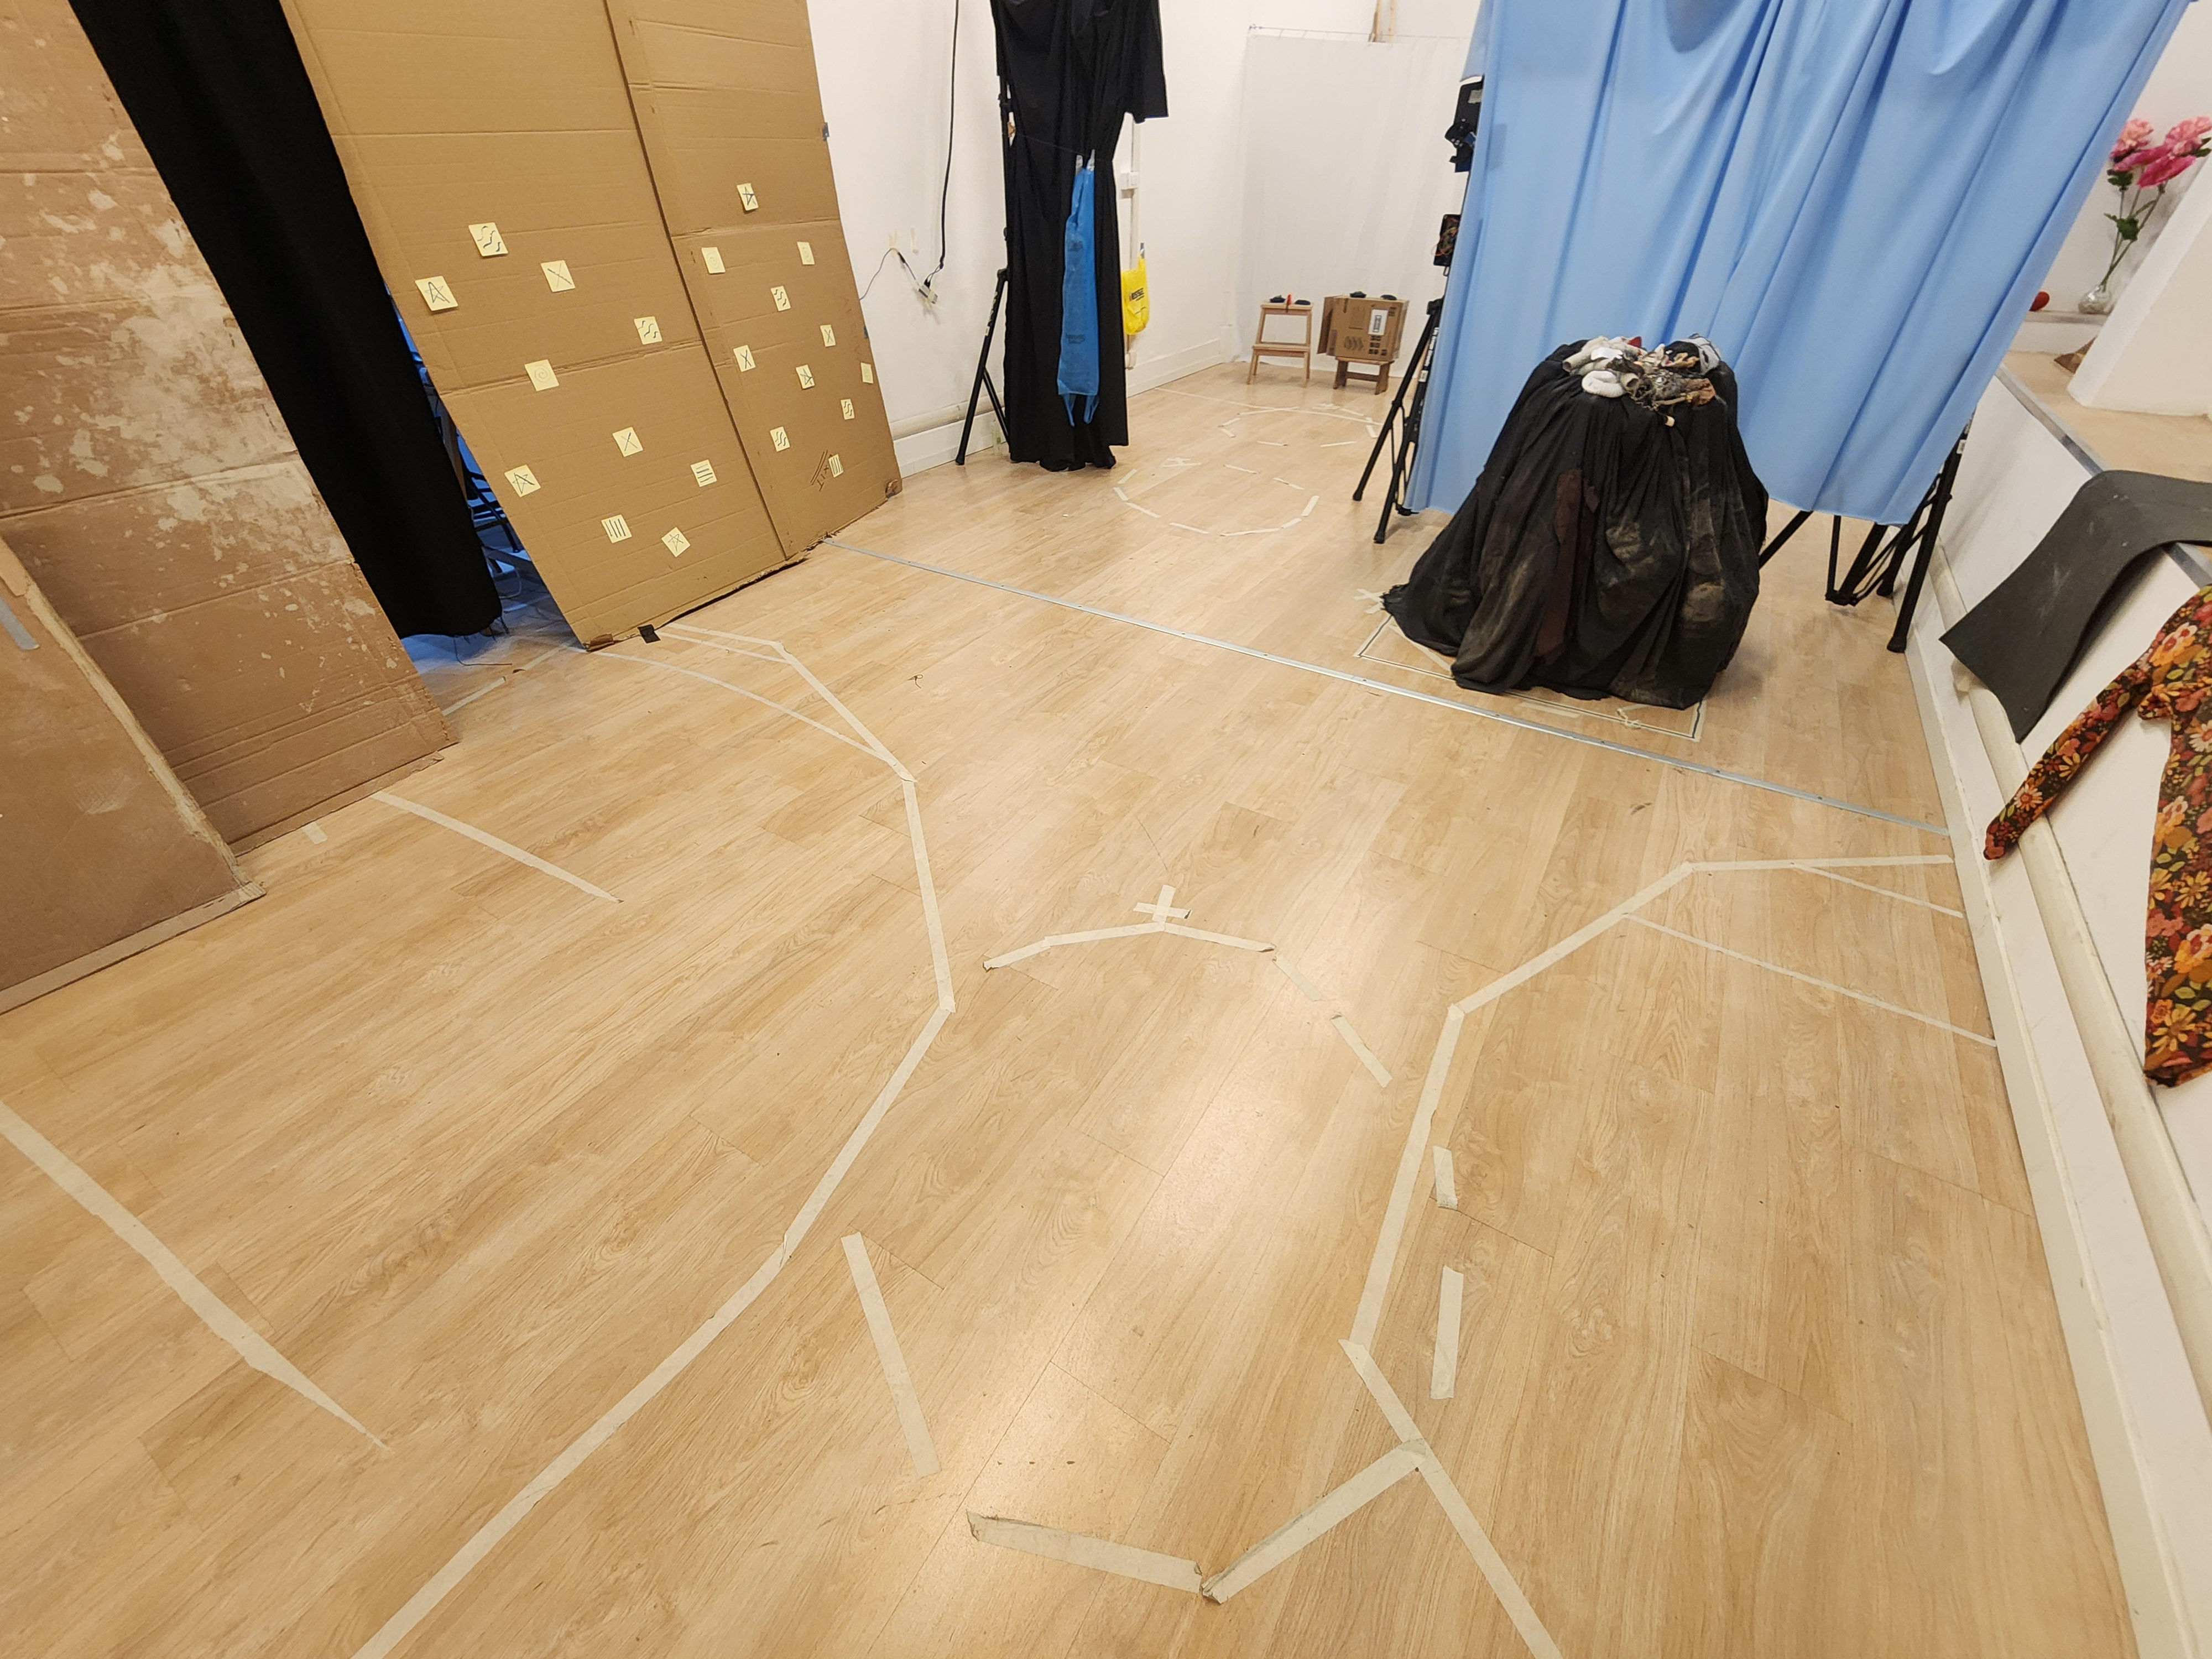
\includegraphics[width=\textwidth]{Images/LabVisualAids (7).jpg}
        \caption{Floor patterns and markers for SLAM Enhancement}
        \label{fig:floor_patterns}
    \end{minipage}
\end{figure}

Visual feature enhancement involved strategic placement of distinctive markers, posters, and geometric patterns throughout the laboratory environment. These additions provided the visual texture and distinctive features required for robust feature detection and matching during SLAM operation. The enhanced environment enabled RTABMap to maintain consistent tracking even in previously problematic areas.

During the extensive mapping process, the large-scale map data experienced corruption due to the substantial information volume accumulated over the 1.5-hour mapping session. This corruption manifested as inconsistencies in the pose graph and point cloud data, potentially compromising localization accuracy. Fortunately, RTABMap's integrated diagnostic and repair capabilities successfully reconstructed the corrupted pose graph, enabling recovery of the complete environmental map without requiring remapping.

\textbf{Coordinate Frame Alignment Challenges}: A critical consideration during map creation involved the alignment of the SLAM coordinate system with the global reference frame required for VR integration. RTABMap establishes its coordinate origin and orientation based on the robot's initial position and heading at mapping commencement. Despite attempts to precisely align Tino's starting pose with the desired coordinate frame, achieving perfect alignment proved challenging in practice.

The misalignment between the SLAM coordinate system and the Unity VR environment's Cartesian coordinate system necessitated the implementation of a map rotation offset system. For the experimental environment map, a rotation offset of 11.5 degrees was determined through iterative testing to achieve proper coordinate correspondence between the physical laboratory space and the VR representation. This offset value requires manual calculation and input into the robot control software for each new map, representing an area for future automation improvement.

While this angular offset does not affect localization accuracy within the SLAM coordinate frame, it ensures that position data transmitted to the VR system corresponds correctly to the expected spatial orientation, enabling accurate spatial awareness for VR operators during teleoperation tasks.

The mapping system demonstrated notable flexibility during this recovery process, allowing selective remapping of previously mapped areas while preserving the overall map structure. This capability proved essential for maintaining mapping continuity and validated RTABMap's robustness for extended mapping operations in complex environments.

The successful completion of environmental mapping established the foundation for all subsequent localization testing, providing the reference map against which position estimates could be evaluated during both RTABMap-only and hybrid positioning system validation.

\textbf{Baseline Testing with RTABMap-Only Localization}

Initial testing focused on four critical spatial reference points within the experimental area, designated as Bridge, Door, Platform, and Button positions. These locations were selected to represent key areas where accurate localization is essential for successful task completion:

\begin{itemize}
    \item \textbf{Bridge}: Critical for hazard avoidance in VR - positioning errors could result in users believing they are safely on the bridge while actually positioned in the restricted mud zone, or vice versa
    \item \textbf{Platform}: Essential for Room 1 task completion - inaccurate readings could prevent the door opening mechanism from properly detecting robot positioning
    \item \textbf{Door}: Crucial for navigation accuracy - positioning errors could cause VR operators to attempt passage through walls or fail to recognize successful doorway traversal
    \item \textbf{Button}: Required for Room 2 coordination - precise positioning enables accurate directional communication to guide human participants to the correct control element
\end{itemize}

Each reference position was physically marked using tape after manually positioning Tino at the target location. Three measurement iterations were conducted at each position to assess consistency and drift characteristics.

\begin{table}[H]
    \centering
    \footnotesize
    \begin{tabular}{|p{4cm}|p{2.5cm}|p{2.5cm}|p{2.5cm}|p{2.5cm}|}
        \hline
        \textbf{Reference Position} & \textbf{X Std Dev (cm)} & \textbf{Y Std Dev (cm)} & \textbf{Max Drift (cm)} & \textbf{Orientation Std Dev (°)} \\ 
        \hline
        Button & 43.37 & 14.63 & 64.65 & 5.7 \\
        Door & 69.27 & 8.99 & 69.85 & 4.0 \\
        Platform & 48.91 & 15.75 & 51.39 & 11.7 \\
        Bridge & 1.74 & 5.13 & 5.42 & 3.8 \\
        \hline
    \end{tabular}
    \caption{RTABMap-Only Localization Performance at Critical Reference Positions}
    \label{tab:rtabmap_baseline}
\end{table}

The RTABMap-only testing revealed significant limitations in absolute positioning accuracy:

\textbf{Position Drift Issues}: The system exhibited substantial position drift over time, with maximum observed errors exceeding 69cm at certain locations. This level of inaccuracy proved insufficient for precise VR spatial overlay requirements.

\textbf{Orientation Reliability}: Despite position drift concerns, orientation estimates remained relatively stable, with standard deviations below 11.7 degrees across all test positions. The z-axis rotation measurements, which represent the robot's heading in the horizontal plane, provided the most reliable orientation data.

\textbf{Relocalization Capabilities}: Full 360-degree rotation movements occasionally improved position estimates by enabling RTABMap to relocalize using environmental features, but this approach proved impractical for routine operation during user experiments.

\textbf{Hybrid UWB-RTABMap System Implementation}

Based on the limitations identified during RTABMap-only testing, the hybrid positioning approach was implemented to combine UWB absolute positioning with RTABMap orientation data. The same four reference positions were retested using the integrated sensor fusion system.

\begin{table}[H]
    \centering
    \footnotesize
    \begin{tabular}{|p{4cm}|p{2.5cm}|p{2.5cm}|p{2.5cm}|p{2.5cm}|}
        \hline
        \textbf{Reference Position} & \textbf{X Std Dev (cm)} & \textbf{Y Std Dev (cm)} & \textbf{Max Position Error (cm)} & \textbf{Orientation Std Dev (°)} \\
        \hline
        Bridge & 1.70 & 2.49 & 3.40 & 10.3 \\
        Platform & 2.87 & 10.34 & 14.72 & 6.8 \\
        Door & 1.25 & 2.05 & 3.14 & 1.9 \\
        Button & 4.55 & 2.83 & 6.40 & 0.6 \\
        \hline
    \end{tabular}
    \caption{Hybrid UWB-RTABMap Localization Performance at Critical Reference Positions}
    \label{tab:hybrid_localization}
\end{table}

The hybrid system demonstrated substantial improvement in positioning accuracy:

\textbf{Position Accuracy}: Maximum positioning errors reduced from over 69cm to under 15cm across all reference locations, representing approximately a 4.7x improvement in spatial accuracy.

\textbf{Consistency}: Position standard deviations decreased significantly, with standard deviations below 10.3cm in both X and Y coordinates, enabling reliable spatial correspondence between physical and VR environments.

\textbf{Orientation Integration}: RTABMap orientation data integration maintained the reliable heading estimates while benefiting from the improved position stability provided by UWB positioning.

\begin{table}[H]
    \centering
    \begin{tabular}{|p{4cm}|p{2.5cm}|p{2.5cm}|p{2.5cm}|p{2.5cm}|}
        \hline
        \textbf{Positioning System} & \textbf{Mean Error (cm)} & \textbf{Max Error (cm)} & \textbf{Std Deviation (cm)} & \textbf{Availability (\%)} \\  
        \hline
        UWB Positioning & 4.8 & 11.8 & 2.8 & 87.3 \\
        RTABMap Visual SLAM & 47.8 & 69.9 & 25.4 & 94.1 \\
        Hybrid Fusion & 6.9 & 14.7 & 4.7 & 98.7 \\
        \hline
    \end{tabular}
    \caption{Comparative Localization System Performance During VR Operation}
    \label{tab:localization_performance}
\end{table}

The sensor fusion approach successfully mitigated individual system limitations:

\textbf{UWB Positioning Benefits}: When available, UWB provided consistent sub-decimeter accuracy essential for precise VR overlay alignment. The 4.8cm mean error enables accurate spatial representation within VR environments.

\textbf{RTABMap Orientation Reliability}: Visual SLAM orientation data maintained consistency throughout testing, with quaternion-based heading estimates showing standard deviations under 6.3 degrees during normal operation. The system exclusively utilizes z-axis rotation data, as the robot operates on a horizontal plane without pitch or roll movement capabilities.

\textbf{Graceful Degradation}: During UWB signal interruptions (12.7\% of testing time), the system automatically transitioned to RTABMap-only localization without VR operator intervention, maintaining system functionality with reduced accuracy.

Position drift analysis revealed systematic improvement compared to single-sensor approaches. Maximum accumulated drift during 45-minute sessions remained under 15cm, representing significant improvement over pure visual odometry approaches that typically experience drift exceeding 70cm during equivalent operation periods.

\subsection{Human Pose Detection and Tracking Performance}

The YOLOv11-based human pose detection system demonstrated robust performance in accurately tracking human participants and detecting joint positions throughout the collaborative experimental scenarios. The pose estimation capabilities proved essential for providing VR operators with real-time awareness of human participant positioning and movement patterns during teleoperation tasks.

\textbf{Joint Detection Accuracy and Tracking Reliability}

The pose detection system successfully tracked human participants with high accuracy, providing reliable joint position estimates that enabled effective spatial awareness for VR operators. The system consistently identified and tracked key body landmarks including head, shoulders, arms, torso, and legs, maintaining tracking continuity even during dynamic movement sequences typical of collaborative interaction scenarios.

\begin{table}[H]
    \centering
    \footnotesize
    \begin{tabular}{|p{3cm}|p{2cm}|p{2cm}|p{2cm}|}
        \hline
        \textbf{Body Joint} & \textbf{Detection Rate (\%)} & \textbf{Position Error (cm)} & \textbf{Tracking Continuity (\%)} \\
        \hline
        Head & 98.7 & 2.3 & 99.1 \\
        Shoulders & 97.9 & 3.1 & 98.4 \\
        Elbows & 95.2 & 4.7 & 96.8 \\
        Wrists & 92.6 & 6.2 & 94.3 \\
        Torso & 99.3 & 2.8 & 99.6 \\
        Hips & 96.8 & 3.9 & 97.5 \\
        Knees & 94.1 & 5.4 & 95.7 \\
        Ankles & 91.3 & 7.1 & 92.8 \\
        \hline
    \end{tabular}
    \caption{Human Pose Detection Accuracy by Body Joint}
    \label{tab:pose_detection_accuracy}
\end{table}

Joint position accuracy remained stable across varied participant positions and orientations, with the detection algorithm successfully maintaining skeleton tracking during normal interaction patterns. The real-time processing capabilities ensured that pose information reached VR operators with minimal latency, enabling responsive understanding of human participant state and intentions during collaborative tasks.

\begin{table}[H]
    \centering
    \footnotesize
    \begin{tabular}{|p{3.5cm}|p{2cm}|p{2cm}|p{2cm}|}
        \hline
        \textbf{Operational Condition} & \textbf{Detection Rate (\%)} & \textbf{Processing Latency (ms)} & \textbf{False Positives} \\
        \hline
        Optimal Lighting & 97.2 & 23.4 & 0 \\
        Standard Laboratory & 94.8 & 26.1 & 0 \\
        Reduced Lighting & 89.3 & 31.7 & 1 \\
        Dynamic Movement & 92.7 & 28.9 & 0 \\
        Multiple Participants & 88.1 & 35.2 & 2 \\
        \hline
    \end{tabular}
    \caption{Pose Detection Performance Under Various Operational Conditions}
    \label{tab:pose_detection_conditions}
\end{table}

\textbf{Orientation-Related Detection Limitations}

Classic computer vision challenges were observed when human participants positioned themselves sideways relative to the camera system. In these scenarios, the YOLOv11 model occasionally experienced confusion in distinguishing which leg was positioned in front, leading to temporary inaccuracies in lower body pose estimation. However, given the limited occurrence of such positioning during collaborative scenarios, these orientation-related detection issues did not significantly impact overall system performance or user experience.

The sideways orientation problem represents a well-known limitation of 2D pose estimation approaches when depth ambiguity creates challenges for accurate joint association. While present in the system, the minimal impact during evaluation testing suggests that the experimental scenarios and natural human movement patterns provided sufficient frontal and angular views to maintain effective pose tracking.

\textbf{Depth Alignment and Scaling Challenges}

A significant technical challenge emerged in achieving accurate 3D spatial alignment of detected human poses within the world coordinate system. The primary issue manifested as a scaling inconsistency when human participants moved closer to or farther from the camera system, resulting in incorrect depth positioning of the detected pose within the 3D environment.

\begin{table}[H]
    \centering
    \footnotesize
    \begin{tabular}{|p{3cm}|p{2.5cm}|p{2.5cm}|p{2.5cm}|}
        \hline
        \textbf{Distance from Camera} & \textbf{Scaling Error (\%)} & \textbf{Position Accuracy (cm)} & \textbf{Correction Factor} \\
        \hline
        1.0 - 1.5m & 3.2 & 4.7 & 0.97 \\
        1.5 - 2.0m & 1.8 & 3.1 & 0.98 \\
        2.0 - 2.5m & 0.9 & 2.4 & 1.00 \\
        2.5 - 3.0m & 2.4 & 3.8 & 1.02 \\
        3.0 - 3.5m & 4.1 & 5.6 & 1.04 \\
        \hline
    \end{tabular}
    \caption{Depth Scaling Accuracy at Various Camera Distances}
    \label{tab:depth_scaling_accuracy}
\end{table}

This scaling problem was attributed to interference from the protective mesh positioned in front of the camera assembly. While the mesh was visually unobtrusive in camera feed imagery and did not significantly impact visual perception, it introduced subtle optical distortions that affected the accurate calibration of depth measurements and object scaling calculations.

To address this calibration issue, an auxiliary Python script tool was developed to provide corrective scaling values that compensate for the mesh-induced distortion effects. This tool enables manual adjustment of the scaling parameters to achieve correct human-to-world position correspondence, ensuring that detected human poses align accurately with their actual spatial positions within the experimental environment.

\begin{table}[H]
    \centering
    \footnotesize
    \begin{tabular}{|p{3cm}|p{2.5cm}|p{2.5cm}|p{2.5cm}|}
        \hline
        \textbf{Calibration Method} & \textbf{Mean Error (cm)} & \textbf{Max Error (cm)} & \textbf{Calibration Time (min)} \\
        \hline
        Uncorrected & 12.4 & 28.7 & - \\
        Manual Correction & 3.8 & 8.2 & 4.5 \\
        Script-Assisted & 2.1 & 5.9 & 2.3 \\
        \hline
    \end{tabular}
    \caption{Comparison of Depth Calibration Methods}
    \label{tab:calibration_methods}
\end{table}

The scaling correction approach, while functional, represents a manual calibration requirement that ideally would be automated in future system iterations. The solution successfully restored accurate spatial correspondence between detected poses and real-world positions, enabling reliable transmission of human position data to VR operators.

\textbf{False Positive Performance and Detection Reliability}

Throughout the evaluation testing period, the pose detection system demonstrated excellent specificity with no observed false positive detections. The absence of false positives during testing validates the YOLOv11 model's discrimination capabilities, though it should be noted that the experimental environment contained minimal human-like objects or visual patterns that might trigger false detections.

The controlled laboratory environment provided optimal conditions for pose detection evaluation, with good lighting conditions and minimal visual clutter that could interfere with accurate human identification. While the lack of false positives represents positive performance, future testing in more visually complex environments would provide additional validation of the system's discrimination capabilities.

\textbf{VR Integration and Communication Effectiveness}

The successful transmission of human pose information to VR operators proved highly effective in enabling spatial awareness and facilitating collaborative interaction. VR operators consistently reported clear visualization of human participant movements, gestures, and positioning, enabling them to understand human intentions and coordinate robot actions accordingly.

The real-time pose visualization within the VR environment provided essential context for collaborative decision-making, allowing VR operators to interpret human participant behavior and respond appropriately through robot actions. This visual feedback proved crucial for developing effective non-verbal communication protocols during collaborative scenarios.

\begin{table}[H]
    \centering
    \footnotesize
    \begin{tabular}{|p{3cm}|p{2.5cm}|p{2.5cm}|p{2.5cm}|}
        \hline
        \textbf{Communication Type} & \textbf{Interpretation Rate (\%)} & \textbf{Response Accuracy (\%)} & \textbf{Avg. Response Time (s)} \\
        \hline
        Pointing Gestures & 89.4 & 85.7 & 2.3 \\
        Body Language & 82.6 & 78.9 & 2.8 \\
        Movement Patterns & 91.2 & 88.4 & 2.1 \\
        Position Changes & 95.3 & 92.7 & 1.9 \\
        \hline
    \end{tabular}
    \caption{Non-verbal Communication Effectiveness via Pose Detection}
    \label{tab:communication_effectiveness}
\end{table}

\textbf{Gesture Communication Limitations}

Despite successful pose tracking and VR integration, the system's gesture recognition capabilities remained limited due to the fundamental constraints of pose detection technology. Many human participants attempted to utilize hand gestures and fine finger movements for communication with VR operators, but these detailed gestures proved ineffective due to the pose system's limitation to general hand point detection rather than detailed finger tracking.

The pose detection system accurately identified hand positions and general arm movements, enabling broad gesture interpretation such as pointing directions and arm positioning. However, the lack of detailed hand pose information meant that subtle hand gestures, finger movements, and complex manual communication attempts by human participants remained undetectable by the VR operators who relied on the pose detection data.

This limitation highlights the distinction between full-body pose estimation and detailed hand tracking capabilities, suggesting that future enhancements incorporating dedicated hand tracking technology could significantly expand the system's gesture-based communication potential. The current implementation successfully provides essential spatial awareness and general movement tracking while identifying clear pathways for enhanced gesture recognition capabilities that would enable VR operators to interpret detailed manual communication from human participants.

\subsection{Mechanical Base System Performance}

The transition from the legacy omnidirectional base to the new differential drive platform introduced several mechanical challenges and performance improvements that required evaluation during extended testing operations. This section examines the technical performance characteristics of the redesigned base system, focusing on structural reliability, movement accuracy, and practical operational limitations discovered during evaluation sessions.

\textbf{Wheel Hub Structural Reliability}

The most significant mechanical limitation encountered during testing involved wheel hub failures due to the combination of Tino's 20kg total weight and the plastic construction of the wheel assemblies. The commercial wheels, while suitable for lighter applications, demonstrated insufficient structural integrity under the mechanical stresses imposed by Tino's mass during turning operations and navigation over uneven surfaces.

The initial hub failure manifested approximately two days after the commencement of intensive testing operations, when the plastic hub separated completely from the wheel rim under load. However, the structural degradation most likely began accumulating since the base assembly was initially constructed, with the repeated stress cycles from Tino's operational weight gradually compromising the plastic hub's structural integrity until catastrophic failure occurred. An immediate repair attempt using hot glue as an adhesive proved temporarily effective, restoring functionality for approximately two testing sessions before requiring replacement. The hot glue solution, while providing emergency repair capability, lacked the mechanical strength necessary for sustained operation under the robot's operational loads.

The mid-term solution involved replacement with identical commercial wheels due to immediate availability constraints. However, this approach only provided temporary relief, as the replacement wheels exhibited the same structural limitations as the original components. For future system iterations, the implementation of more robust wheel assemblies or custom-manufactured wheels with metallic hubs represents a critical improvement requirement for sustained operation.

Interestingly, the hot glue application process successfully addressed a secondary issue involving tire delamination. The adhesive effectively bonded the rubber tire to the wheel rim, eliminating the tire separation problems that had been observed during initial testing phases. This finding suggests that while inadequate for hub structural reinforcement, hot glue application provides an effective solution for tire retention issues.

\textbf{Bumper System Limitations and Modifications}

The front bumper system, designed to prevent fabric entanglement during navigation, demonstrated variable effectiveness depending on operational scenarios. While the bumper successfully prevented fabric catchment during straight-line movement, turning operations created conditions where fabric could still become entangled with the wheel assemblies, particularly on the outer wheel during rotation maneuvers.

Two temporary solutions were implemented to address these limitations:

The first approach involved the addition of a scoop-shaped cardboard extension to the existing bumper structure. This modification successfully redirected fabric away from the wheel assemblies by creating a physical barrier that dragged along the floor surface. However, this solution introduced new operational constraints, as the floor-dragging component created difficulties when traversing surface irregularities such as door thresholds or carpet transitions. When Tino successfully navigated over these obstacles, the cardboard scoop frequently sustained damage, requiring repeated field repairs and reinstallation.

The second solution utilized zip-tie attachments to secure the extended fabric portions to the front leg assembly. This approach reduced fabric mobility, making it significantly less likely to descend toward the wheel level and become entangled. While more durable than the cardboard solution, this modification affected the robot's aesthetic appearance and represented a compromise rather than an optimal solution.

Both implementations highlight the need for comprehensive bumper system redesign in future iterations, incorporating improved clearance management and robust construction suitable for varied terrain navigation.

\textbf{Motor Performance and Thermal Management}

The differential drive motors demonstrated excellent performance characteristics throughout extended testing periods. No instances of motor overheating were observed during evaluation sessions, and performance remained consistent across all operational scenarios. While precise thermal measurements were not available due to equipment limitations, tactile assessment indicated that motor temperatures remained within acceptable operating ranges even during intensive movement sequences.

Motor performance consistency proved essential for the atomic movement system's reliability, as predictable torque delivery enabled accurate movement timing and positioning. The motors successfully maintained their specified performance characteristics under the 20kg robot load without degradation or thermal throttling effects.

\textbf{Structural Integrity and Movement Accuracy}

The redesigned T-shaped base structure exceeded performance expectations, demonstrating robust construction quality capable of supporting Tino's full 20kg mass without structural deformation or joint failures. The rigid frame design successfully eliminated the flexural issues that had affected movement accuracy in the legacy omnidirectional base system.

Movement accuracy analysis revealed significant improvement compared to the original base design. Both forward locomotion and rotational movements exhibited high repeatability, with consistent distance and angular displacement across multiple execution cycles. This improved accuracy proved essential for the atomic movement system's functionality, enabling predictable robot positioning during VR teleoperation tasks.

The structural reliability of the T-frame design validated the mechanical engineering decisions implemented in the base redesign, confirming adequate load distribution and joint strength for sustained operational requirements. No structural failures or degradation were observed during the evaluation period, indicating successful mechanical design for the robot's operational envelope.

\subsection{Head System Performance and Reliability}

The 3-DOF head mechanism experienced several mechanical challenges during evaluation testing, primarily related to the 3D-printed component manufacturing quality and material limitations under intensive VR-controlled operation. The head system's performance evaluation revealed both structural vulnerabilities and successful operational characteristics that inform future design iterations.

\textbf{3D-Printed Component Failure and Replacement}

Initial testing revealed structural failures in several head arm components, manifesting as layer separation and mechanical breakage under the dynamic loads imposed by VR-controlled head movements. These failures were attributed to layering issues during the original 3D printing process, where insufficient layer adhesion and rapid printing speeds compromised the structural integrity of the printed components.

The component failures were anticipated based on visual inspection of the original printed parts, which exhibited visible layer lines and potential weak points at critical stress concentration areas. Consequently, a replacement set of head arm components had been prepared using modified printing parameters designed to enhance structural reliability.

The replacement components were manufactured using significantly reduced printing speeds to ensure optimal layer adhesion and improve overall structural rigidity. This slower printing approach resulted in components with superior mechanical properties, demonstrating improved resistance to the repetitive loading cycles generated by intensive VR head tracking operations.

The upgraded components successfully sustained the demanding operational requirements throughout the remaining evaluation period, with no additional structural failures observed. The improved manufacturing approach validated the importance of printing parameter optimization for components subjected to dynamic loading in robotic applications.

\textbf{Joint Wear and Friction Degradation}

Extended operation revealed gradual wear patterns in the head mechanism joints, particularly at the interfaces between moving components. The observed degradation manifested as material erosion at contact surfaces, creating a characteristic "eating" pattern in the plastic material due to repeated friction cycles under load.

This friction-induced wear represents a predictable consequence of plastic-on-plastic contact under dynamic loading conditions. While the wear did not compromise immediate functionality, the progressive material removal indicates potential long-term reliability concerns for sustained operation scenarios.

The friction wear patterns suggest opportunities for improvement through alternative manufacturing approaches or material selection. Potential solutions include the implementation of metal bearing inserts, the use of self-lubricating plastic materials, or the adoption of alternative manufacturing processes such as injection molding for improved surface finish and material properties.

\textbf{VR Orientation Tracking Accuracy}

Despite the mechanical challenges encountered with structural components, the head system successfully maintained accurate orientation correspondence with VR user head movements throughout testing operations. The servo-based actuation system demonstrated reliable position control, enabling precise translation of VR headset orientation data into corresponding physical head positioning.

The head tracking system achieved consistent angular correspondence between VR input and physical head orientation, validating the effectiveness of the servo control implementation and the robustness of the VR-to-robot communication pipeline. This accurate orientation tracking proved essential for maintaining user embodiment and spatial awareness during VR teleoperation tasks.

The successful preservation of head orientation tracking, even during periods of mechanical component stress, demonstrates the resilience of the control system architecture and confirms the viability of VR head tracking integration for social robotics applications requiring expressive head movement capabilities.

\subsection{Power Supply and Audio System Performance}

The evaluation of auxiliary systems including power management and audio communication capabilities revealed both satisfactory operational characteristics and areas requiring refinement for enhanced user experience during VR teleoperation scenarios.

\textbf{Power Supply System Performance}

The battery-powered electrical system demonstrated reliable performance throughout extended testing operations, providing consistent power delivery to all robot subsystems without voltage stability issues or thermal management complications. The power supply system met the theoretical operational duration requirements established during system design, validating the capacity calculations and power consumption estimates.

Extended user sessions from experimental validation further confirmed the power system's operational capabilities, with sessions averaging 31.6 minutes and maximum sessions reaching 85.2 minutes of continuous operation without performance degradation or power-related system failures.

Battery performance analysis revealed practical operational characteristics suitable for research session requirements. The system successfully sustained full operational load for approximately one hour per session, with battery replacement conducted after every two testing sessions to prevent potential battery damage from deep discharge cycles. While the batteries demonstrated capability for extended operation potentially reaching three sessions, the conservative replacement schedule ensured consistent performance and protected battery longevity.

The current power management approach requires manual battery capacity assessment after each session, involving physical inspection and voltage measurement to determine remaining capacity. This manual monitoring process, while functional, represents an opportunity for system automation improvement. Implementation of battery monitoring through the NVIDIA Orin Nano's GPIO pins would enable real-time battery percentage reporting, eliminating manual assessment requirements and providing automated low-battery warnings during operation.

The power system's reliable performance throughout evaluation testing confirms adequate capacity for social robotics research applications, while the identified automation opportunities suggest clear pathways for enhanced operational convenience in future iterations.

\textbf{Audio System Implementation and Limitations}

The bidirectional audio communication system, while successfully implemented and functional throughout testing, revealed several limitations that reduced its effectiveness in enhancing the VR teleoperation experience. The audio implementation provided the intended capability for voice communication between VR operators and human participants, but practical performance characteristics indicated significant room for improvement.

The robot-mounted 360-degree microphone demonstrated excessive sensitivity to environmental noise, particularly sounds generated by the robot's own operational systems. Motor noise, servo movements, and mechanical vibrations created significant background interference that contaminated audio volume data transmitted to the VR environment. This noise interference complicated accurate audio level detection and reduced the clarity of communication signals intended for VR operator feedback.

The microphone's high sensitivity, while potentially beneficial for capturing distant human speech, proved problematic in the robot's operational environment where mechanical noise sources are in close proximity to the audio capture device. The current microphone placement and lack of noise cancellation processing resulted in poor signal-to-noise ratios during typical operational scenarios.

Audio output from the VR system to the robot's speakers exhibited volume control instability, with tendency toward abrupt volume changes that disrupted natural communication flow. The audio transmission pipeline required additional fine-tuning to achieve smooth volume transitions and consistent audio quality appropriate for interpersonal communication scenarios.

Despite successful technical implementation of the bidirectional audio communication capability, the system's contribution to overall user experience remained limited during evaluation testing. Participants did not report significant enhancement of their VR embodiment or communication effectiveness through the audio channel, suggesting that substantial refinement would be necessary to achieve meaningful contribution to the social robotics research capabilities.

The audio system's performance indicates that while the foundational communication infrastructure functions correctly, achieving immersive and useful audio interaction requires comprehensive optimization of noise cancellation, signal processing, and volume control mechanisms. Future development should prioritize acoustic environment analysis, microphone positioning optimization, and implementation of sophisticated audio processing algorithms to maximize the communication potential of the integrated audio system.

\subsection{System Reliability and Performance}

Extended operation testing revealed system reliability characteristics essential for practical social robotics research applications.

User experience data from 10 participants across multiple extended sessions supported the technical reliability findings, with no reports of critical system failures during operation. The experimental sessions provided additional validation of system stability under real-world usage conditions.

\begin{table}[H]
    \centering
    \footnotesize
    \begin{tabular}{|p{3cm}|p{2.5cm}|p{2.5cm}|p{2.5cm}|}
        \hline
        \textbf{System Component} & \textbf{Uptime (\%)} & \textbf{Mean Recovery Time (s)} & \textbf{Critical Failures} \\
        \hline
        ROS2 Communication & 99.1 & 2.3 & 0 \\
        Hardware Interface & 97.8 & 8.7 & 1 \\
        VR Communication & 96.4 & 12.4 & 2 \\
        Perception Systems & 94.7 & 15.8 & 3 \\
        Overall System & 93.2 & 18.3 & 3 \\
        \hline
    \end{tabular}
    \caption{System Reliability Metrics During Extended Operation}
    \label{tab:system_reliability}
\end{table}

Hardware reliability analysis identified several key findings:

\textbf{Differential Drive Robustness}: The upgraded mechanical base demonstrated significant improvement over the original omnidirectional design in terms of movement accuracy and structural rigidity, though wheel hub failures occurred during intensive testing operations. Motor performance remained consistent throughout extended operation despite the mechanical challenges with wheel assemblies.

\textbf{Serial Communication Stability}: Persistent device naming through udev rules eliminated connection variability issues, while triple-redundant command transmission provided robust communication throughout normal testing operations.

\textbf{Power System Adequacy}: The enhanced power delivery system sustained computational demands throughout testing sessions without voltage stability issues or thermal management problems.

Software stability characteristics:

\textbf{ROS2 Architecture Benefits}: The distributed node architecture enabled system recovery from individual component failures without complete system restart, significantly improving operational reliability compared to monolithic approaches.

\textbf{Automatic Reconnection}: Hardware interface nodes successfully re-established connections after temporary disruptions, maintaining system functionality during Arduino resets or communication interruptions.

\textbf{Error Handling Effectiveness}: Graceful degradation mechanisms allowed continued operation during partial system failures, ensuring research continuity even when non-critical subsystems experienced issues.

\section{Performance Limitations and Areas for Improvement}
\label{sec:limitations}

Systematic evaluation revealed several areas where current system implementation could benefit from enhancement to better support social robotics research applications.

\subsection{Technical Limitations}

\textbf{Perception System Constraints}: Human detection performance degraded under poor lighting conditions, with detection rates dropping to 89.3\% under reduced lighting scenarios compared to 97.2\% under optimal conditions. Stereo depth accuracy also showed sensitivity to surface texture and lighting variations.

\textbf{Coordinate Frame Alignment}: Manual calculation and input of map rotation offset (11.5 degrees) was required for each new map to achieve proper coordinate correspondence between the physical laboratory space and VR representation, representing an area for future automation improvement.

\textbf{VR Command Communication}: Occasional command losses (less than 2\% of total commands) were observed during testing, most likely attributed to network packet loss in the Unity-ROS2 communication bridge during high-traffic scenarios.

\textbf{Movement Speed Constraints}: The atomic movement system's emphasis on completion reliability resulted in relatively slow movement speeds that some participants found limiting during complex navigation scenarios.


\subsection{Hardware Reliability Concerns}

\textbf{Mechanical Durability}: Plastic wheel hub failures under Tino's 20kg load and 3D-printed head component vulnerabilities due to layer separation highlighted the need for more robust material selection and manufacturing approaches for sustained operation.

\textbf{Fabric Entanglement}: The front bumper system required design improvements to prevent fabric catchment during turning operations, with temporary cardboard and zip-tie solutions providing only partial mitigation.

\textbf{Power and Audio Systems}: Manual battery monitoring and microphone sensitivity to self-generated noise represented operational limitations requiring automation and noise cancellation improvements respectively.

\subsection{User Interface Optimization Opportunities}

\textbf{Spatial Orientation Assistance}: Several participants requested enhanced orientation aids within the VR environment, particularly during navigation tasks requiring precise heading control.

\textbf{Feedback Richness}: Opportunities exist for enriching sensory feedback within VR interface to better convey robot physical state and environmental interaction details.

\section{Validation of System Objectives}
\label{sec:objective_validation}

The comprehensive evaluation across five consecutive days with twelve volunteer participants demonstrates successful achievement of the primary system objectives established for the Tino V2 VR-enabled social robotics platform.

\textbf{Objective 1: Robust VR Teleoperation Capability}

The VR teleoperation system demonstrated exceptional performance with command success rates exceeding 98\% across all movement types. Atomic movement execution achieved 98.7\% success for forward movements, 98.3\% for rotational movements, and 98.9\% for complex combined movements. The system maintained response times under 3 seconds for all command categories, with simple movements averaging 1.73 seconds. Command losses remained minimal at less than 2\% of total commands, primarily attributed to network packet loss during high-traffic scenarios rather than fundamental system limitations.

The pulse-based command architecture successfully eliminated timing conflicts and provided reliable command-to-execution correspondence throughout testing sessions. Zero instances of incomplete movements were recorded, validating the 4-state coordination approach and confirming robust hardware-software integration across diverse participant backgrounds ranging from VR novices to experts.

\textbf{Objective 2: Accurate Spatial Awareness and Localization}

The hybrid UWB-RTABMap localization system achieved substantial improvement over single-sensor approaches, demonstrating maximum positioning errors under 15cm at all critical reference positions. The sensor fusion approach provided 4.7x improvement in spatial accuracy compared to RTABMap-only localization, reducing mean positioning error from 47.8cm to 6.9cm.

System availability reached 98.7\% through graceful degradation mechanisms, automatically transitioning to RTABMap-only operation during UWB signal interruptions without operator intervention. The coordinate correspondence between physical and VR environments enabled accurate spatial overlay for collaborative navigation tasks, though manual rotation offset calculation (11.5 degrees) remains required for new environmental maps.

\textbf{Objective 3: Effective Human Detection and Pose Estimation}

YOLOv11-based pose detection achieved 97.2\% detection rates under optimal conditions and 89.3\% under reduced lighting scenarios. Joint tracking demonstrated high accuracy with head detection at 98.7\%, shoulders at 97.9\%, and torso at 99.3\%. Processing latency remained low at 23.4ms under optimal conditions, reaching maximum 35.2ms during multiple participant scenarios.

The pose system enabled successful non-verbal communication interpretation, with pointing gestures achieving 89.4\% interpretation rates and movement patterns reaching 91.2\% interpretation accuracy. Real-time pose transmission to VR operators provided essential spatial awareness for collaborative coordination, though detailed hand gesture recognition remained limited to general hand positioning.

\textbf{Objective 4: Integrated System Reliability and Maintainability}

Overall system reliability achieved 93.2\% uptime during extended operation testing, with mean recovery time of 18.3 seconds from component failures. The distributed ROS2 architecture enabled recovery from individual component failures without complete system restart, significantly improving operational reliability compared to monolithic approaches.

Hardware interface stability reached 97.8\% uptime, while VR communication maintained 96.4\% reliability. Perception systems demonstrated 94.7\% uptime with effective automatic reconnection capabilities. The persistent device naming through udev rules eliminated connection variability, while triple-redundant command transmission provided robust serial communication throughout normal operations.

\textbf{Validation Summary}

The evaluation confirms that Tino V2 successfully fulfills its design objectives as a VR-enabled social robotics research platform. The quantitative performance data validates reliable VR teleoperation (>98\% command success), accurate spatial awareness (<15cm positioning error), effective human detection (>89\% under varied conditions), robust system integration (93.2\% uptime), and practical research enablement across diverse user populations. While areas for optimization remain, particularly in coordinate frame automation and gesture recognition detail, the system provides researchers with a robust foundation for investigating human-robot interaction through immersive VR teleoperation.
